\documentclass[unknownkeysallowed]{beamer}

\usepackage{graphicx}
\usepackage{xcolor}
\usepackage{caption}
\usepackage{subcaption}

\definecolor{highlight-colour}{RGB}{153, 255, 204}

\newcommand{\highlight}[1]{%
  \colorbox{highlight-colour}{$\displaystyle#1$}}

\usetheme{Antibes}
\usecolortheme{lily}

\mode<presentation>

\title[Agency in disease modelling]{Introducing features of agency into computational models of infectious disease}
\author{Ethan Kelly\\ \texttt{e.kelly.1@research.gla.ac.uk}}
\date{27 May 2021}

\begin{document}

% =============================================================================
% Title slide.
{
  \usebackgroundtemplate{
\includegraphics[height=\paperheight]{assets/title-slide}}

  \begin{frame}[plain]
    \setbeamercolor{title}{fg=white}
    \setbeamercolor{author}{fg=white}
    \setbeamercolor{date}{fg=white}

    \begin{columns}

      \begin{column}[l]{3cm}
      \end{column}

      \begin{column}[r]{7cm}
        \titlepage
      \end{column}

    \end{columns}
  \end{frame}
}

% Table of contents.
\begin{frame}
  \frametitle{Outline}
  \tableofcontents
\end{frame}

% =============================================================================
\section{Introduction to Computational Disease Modelling}

% -----------------------------------------------------------------------------

\begin{frame}
  \frametitle{Outline}
  \tableofcontents[currentsection]
\end{frame}

% -----------------------------------------------------------------------------
\subsection{Graph Theory}

\begin{frame}{What is a Graph?}

What is a graph (network)?

  \begin{itemize}
    \pause
  \item A set of objects where some pairs are related.
    \pause
  \item Objects are called {\it vertices} or {\it nodes}
    \pause
  \item Relations between objects are called {\it edges}. 
  \end{itemize}
%  \pause
%  \centering
%  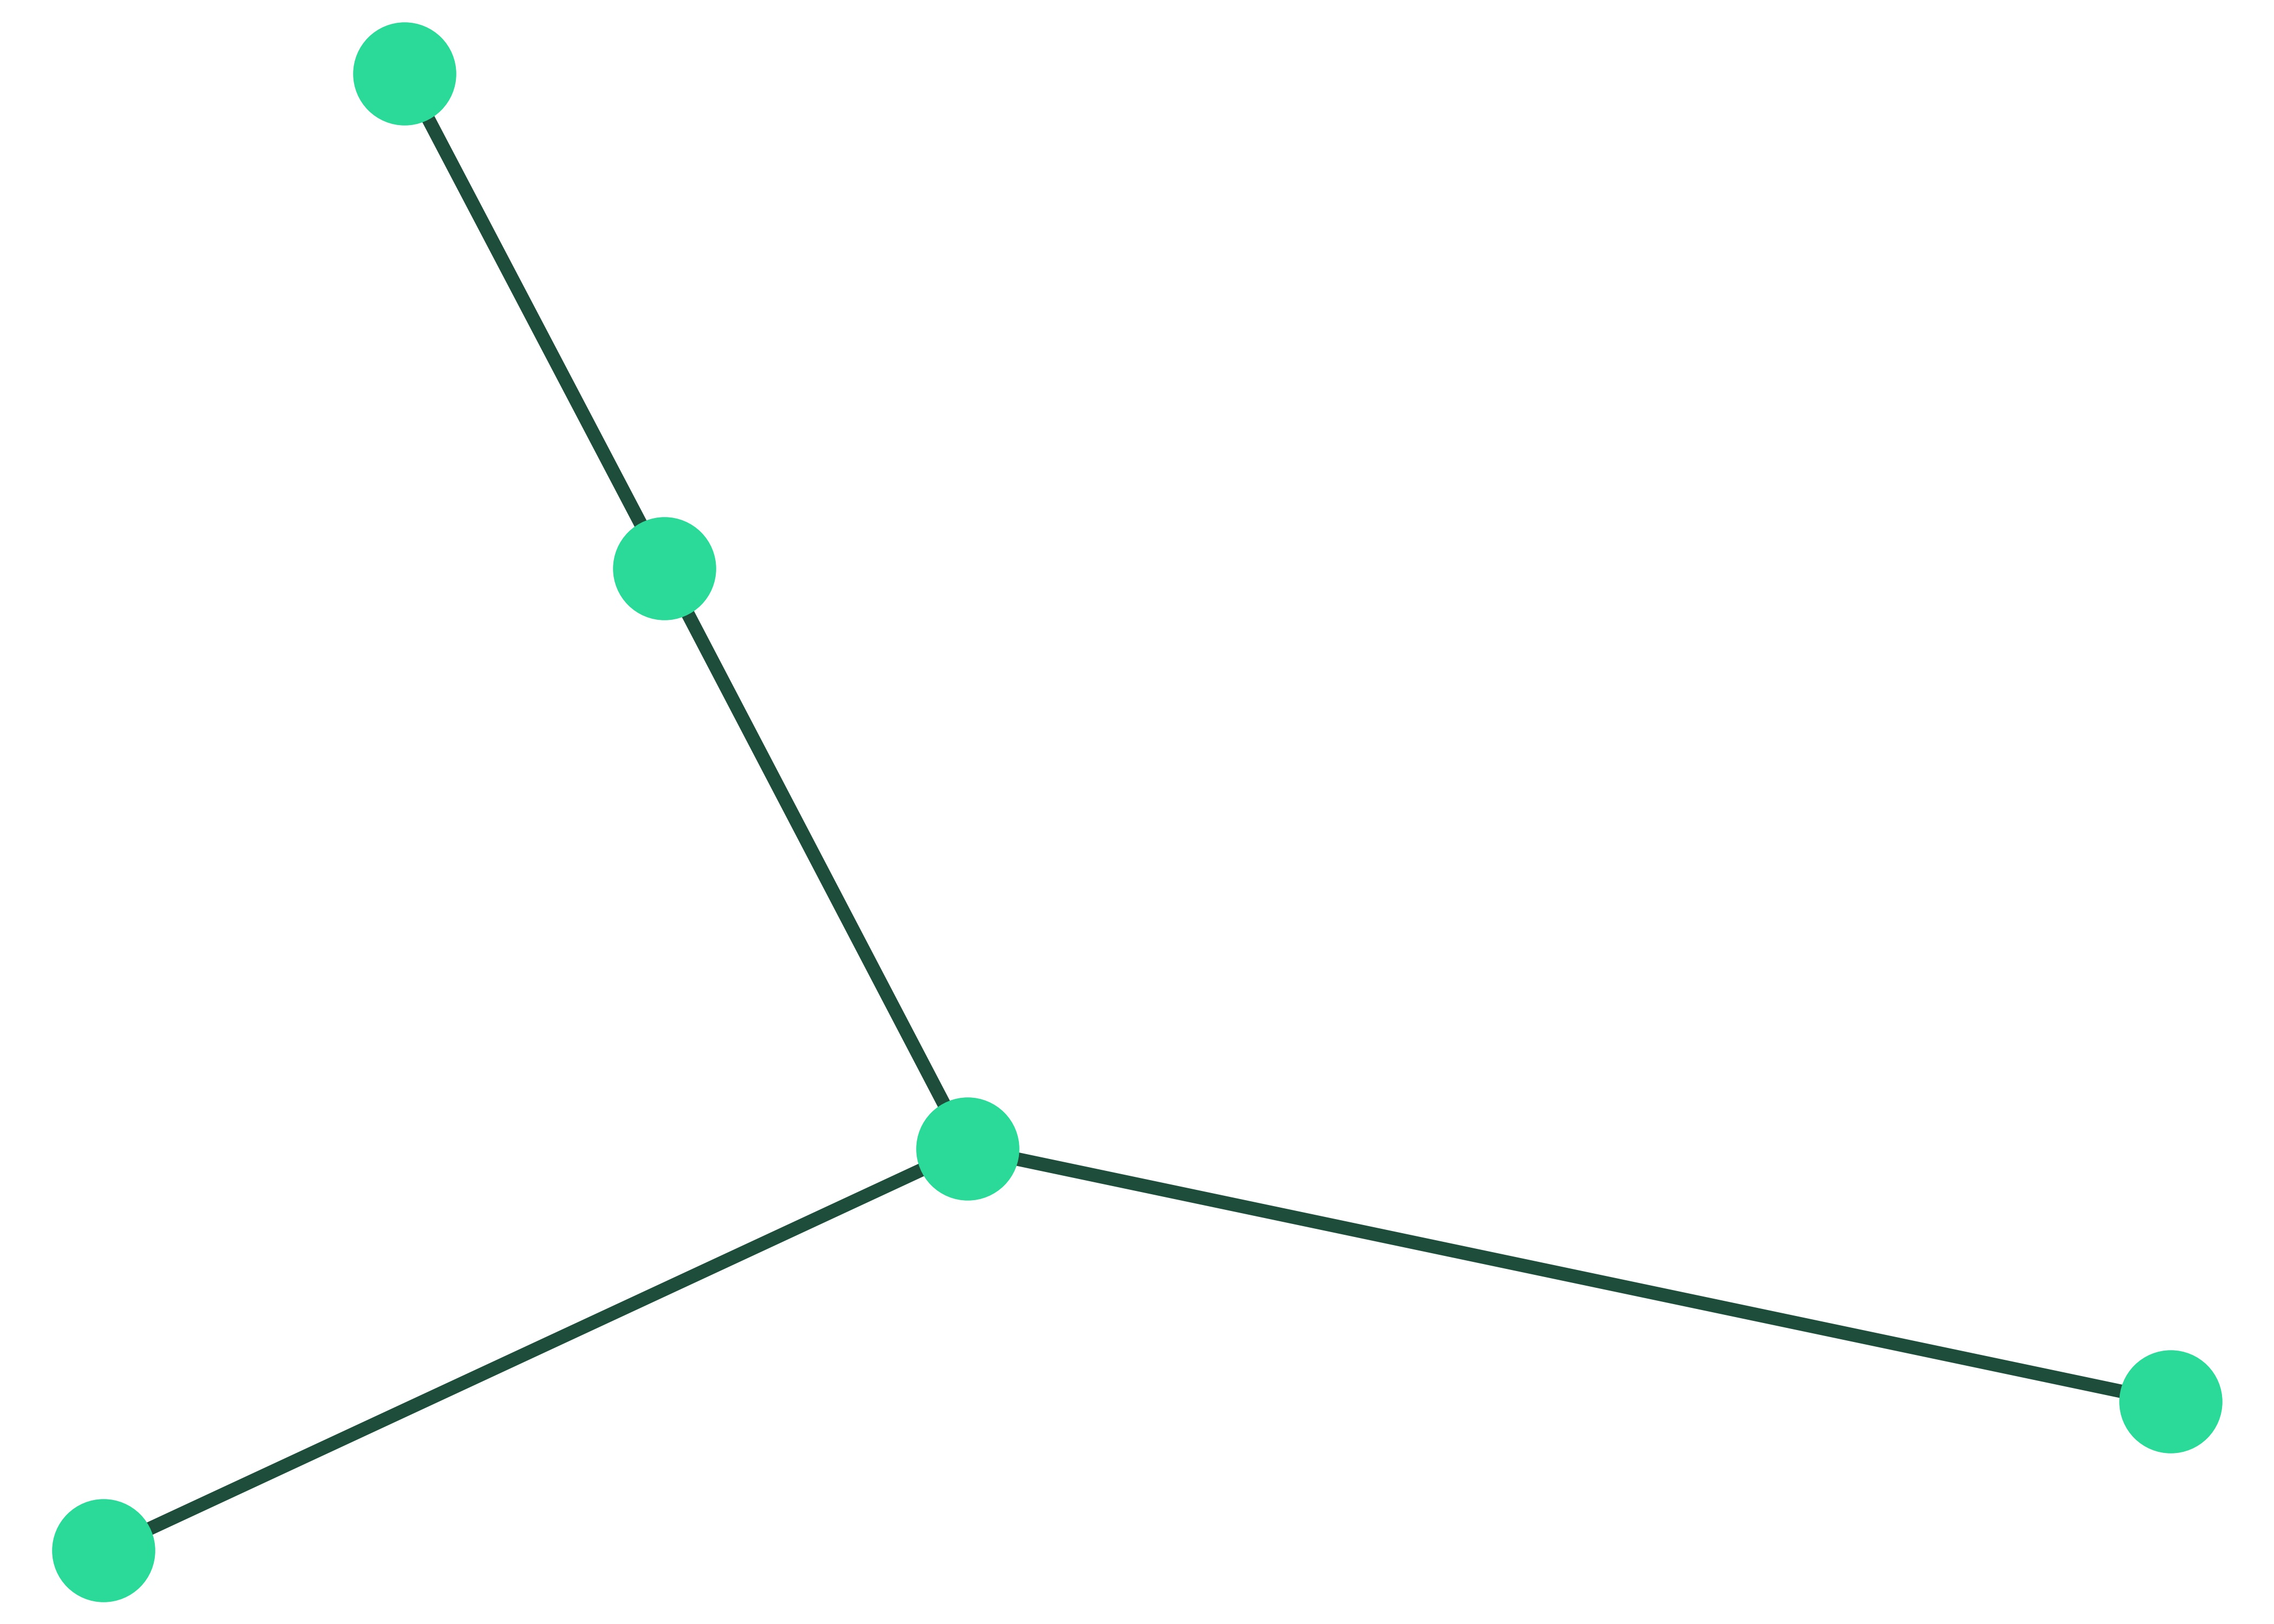
\includegraphics[width=0.5\textwidth]{assets/mini-tree}

\end{frame}
% -----------------------------------------------------------------------------
%\begin{frame}{Examples of Graphs}
%
%\begin{columns}
%
%\begin{column}{.6\textwidth}
%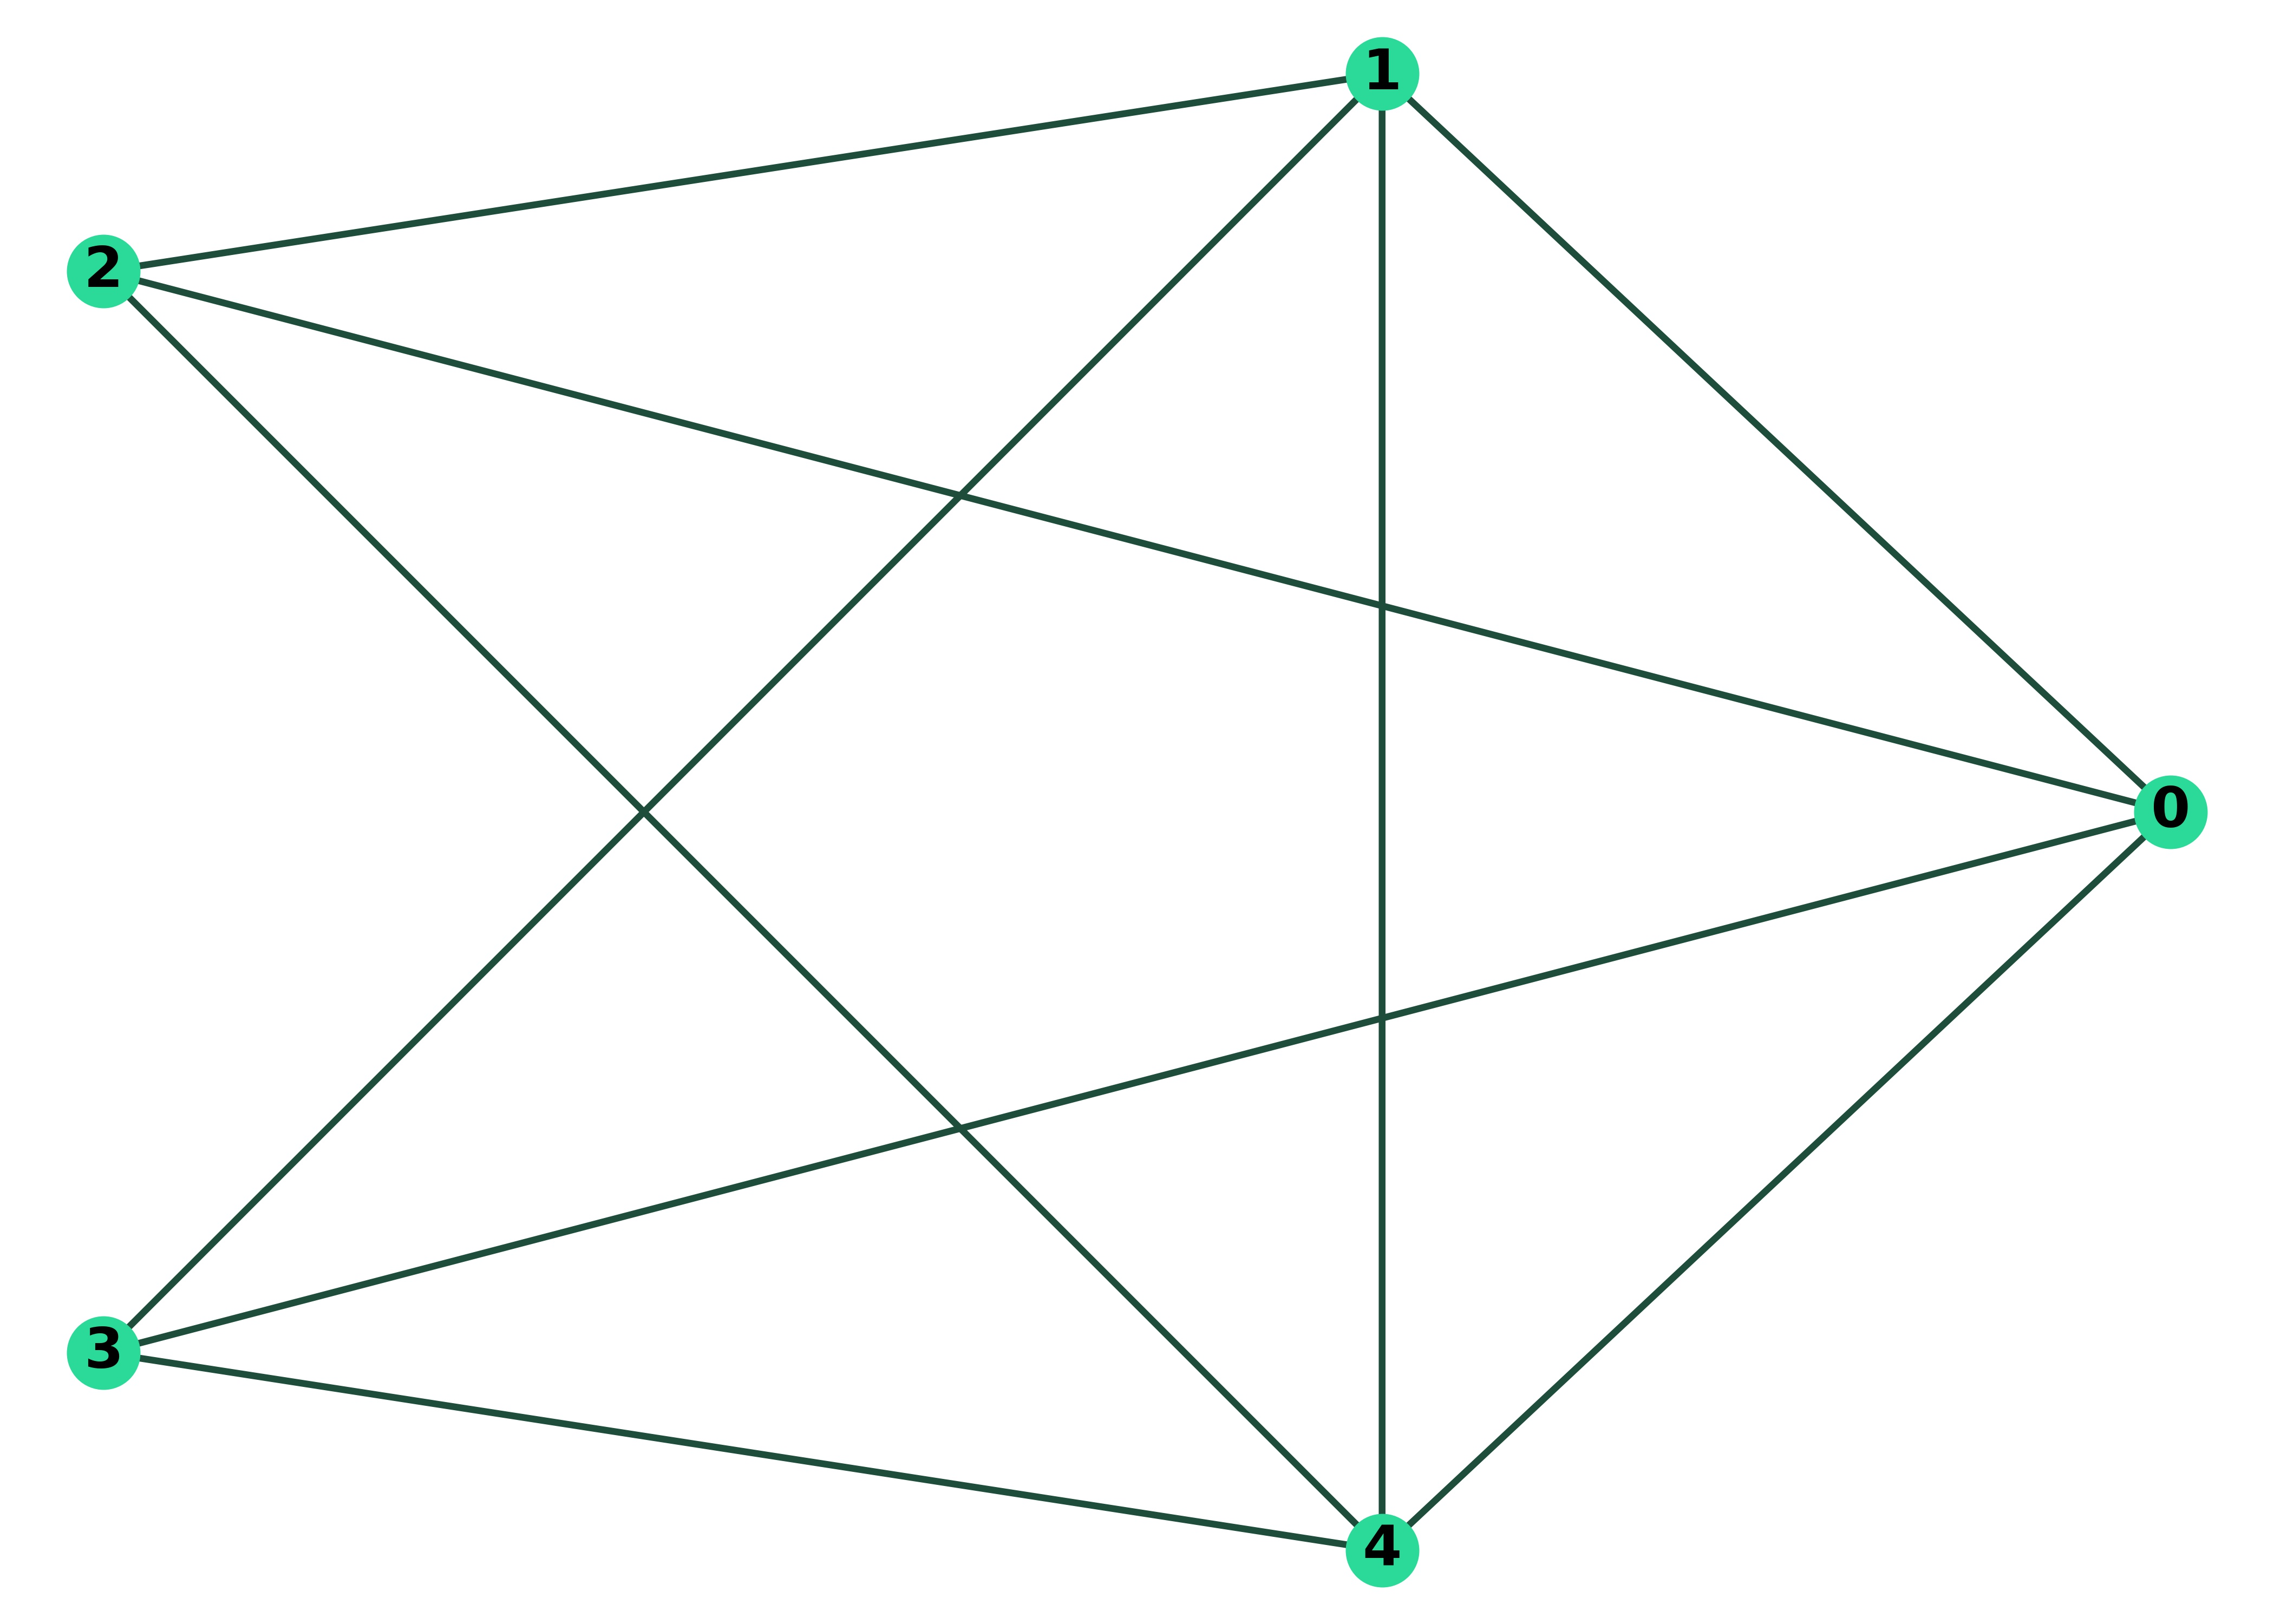
\includegraphics[width=.8\linewidth,valign=t]{assets/er}
%\end{column}
%
%\begin{column}{.4\textwidth}
%\textbf{Example: Erd\H{o}s-R\'{e}nyi}
%
%\vspace{5pt}
%
%Random graph with a given number of vertices (in this case, 5) and a probability with which an edge exists between any two vertices.
%
%\end{column}
%
%\end{columns}
%\end{frame}
% -----------------



\begin{frame}{Examples of Graphs}

\begin{columns}

\begin{column}{.6\textwidth}
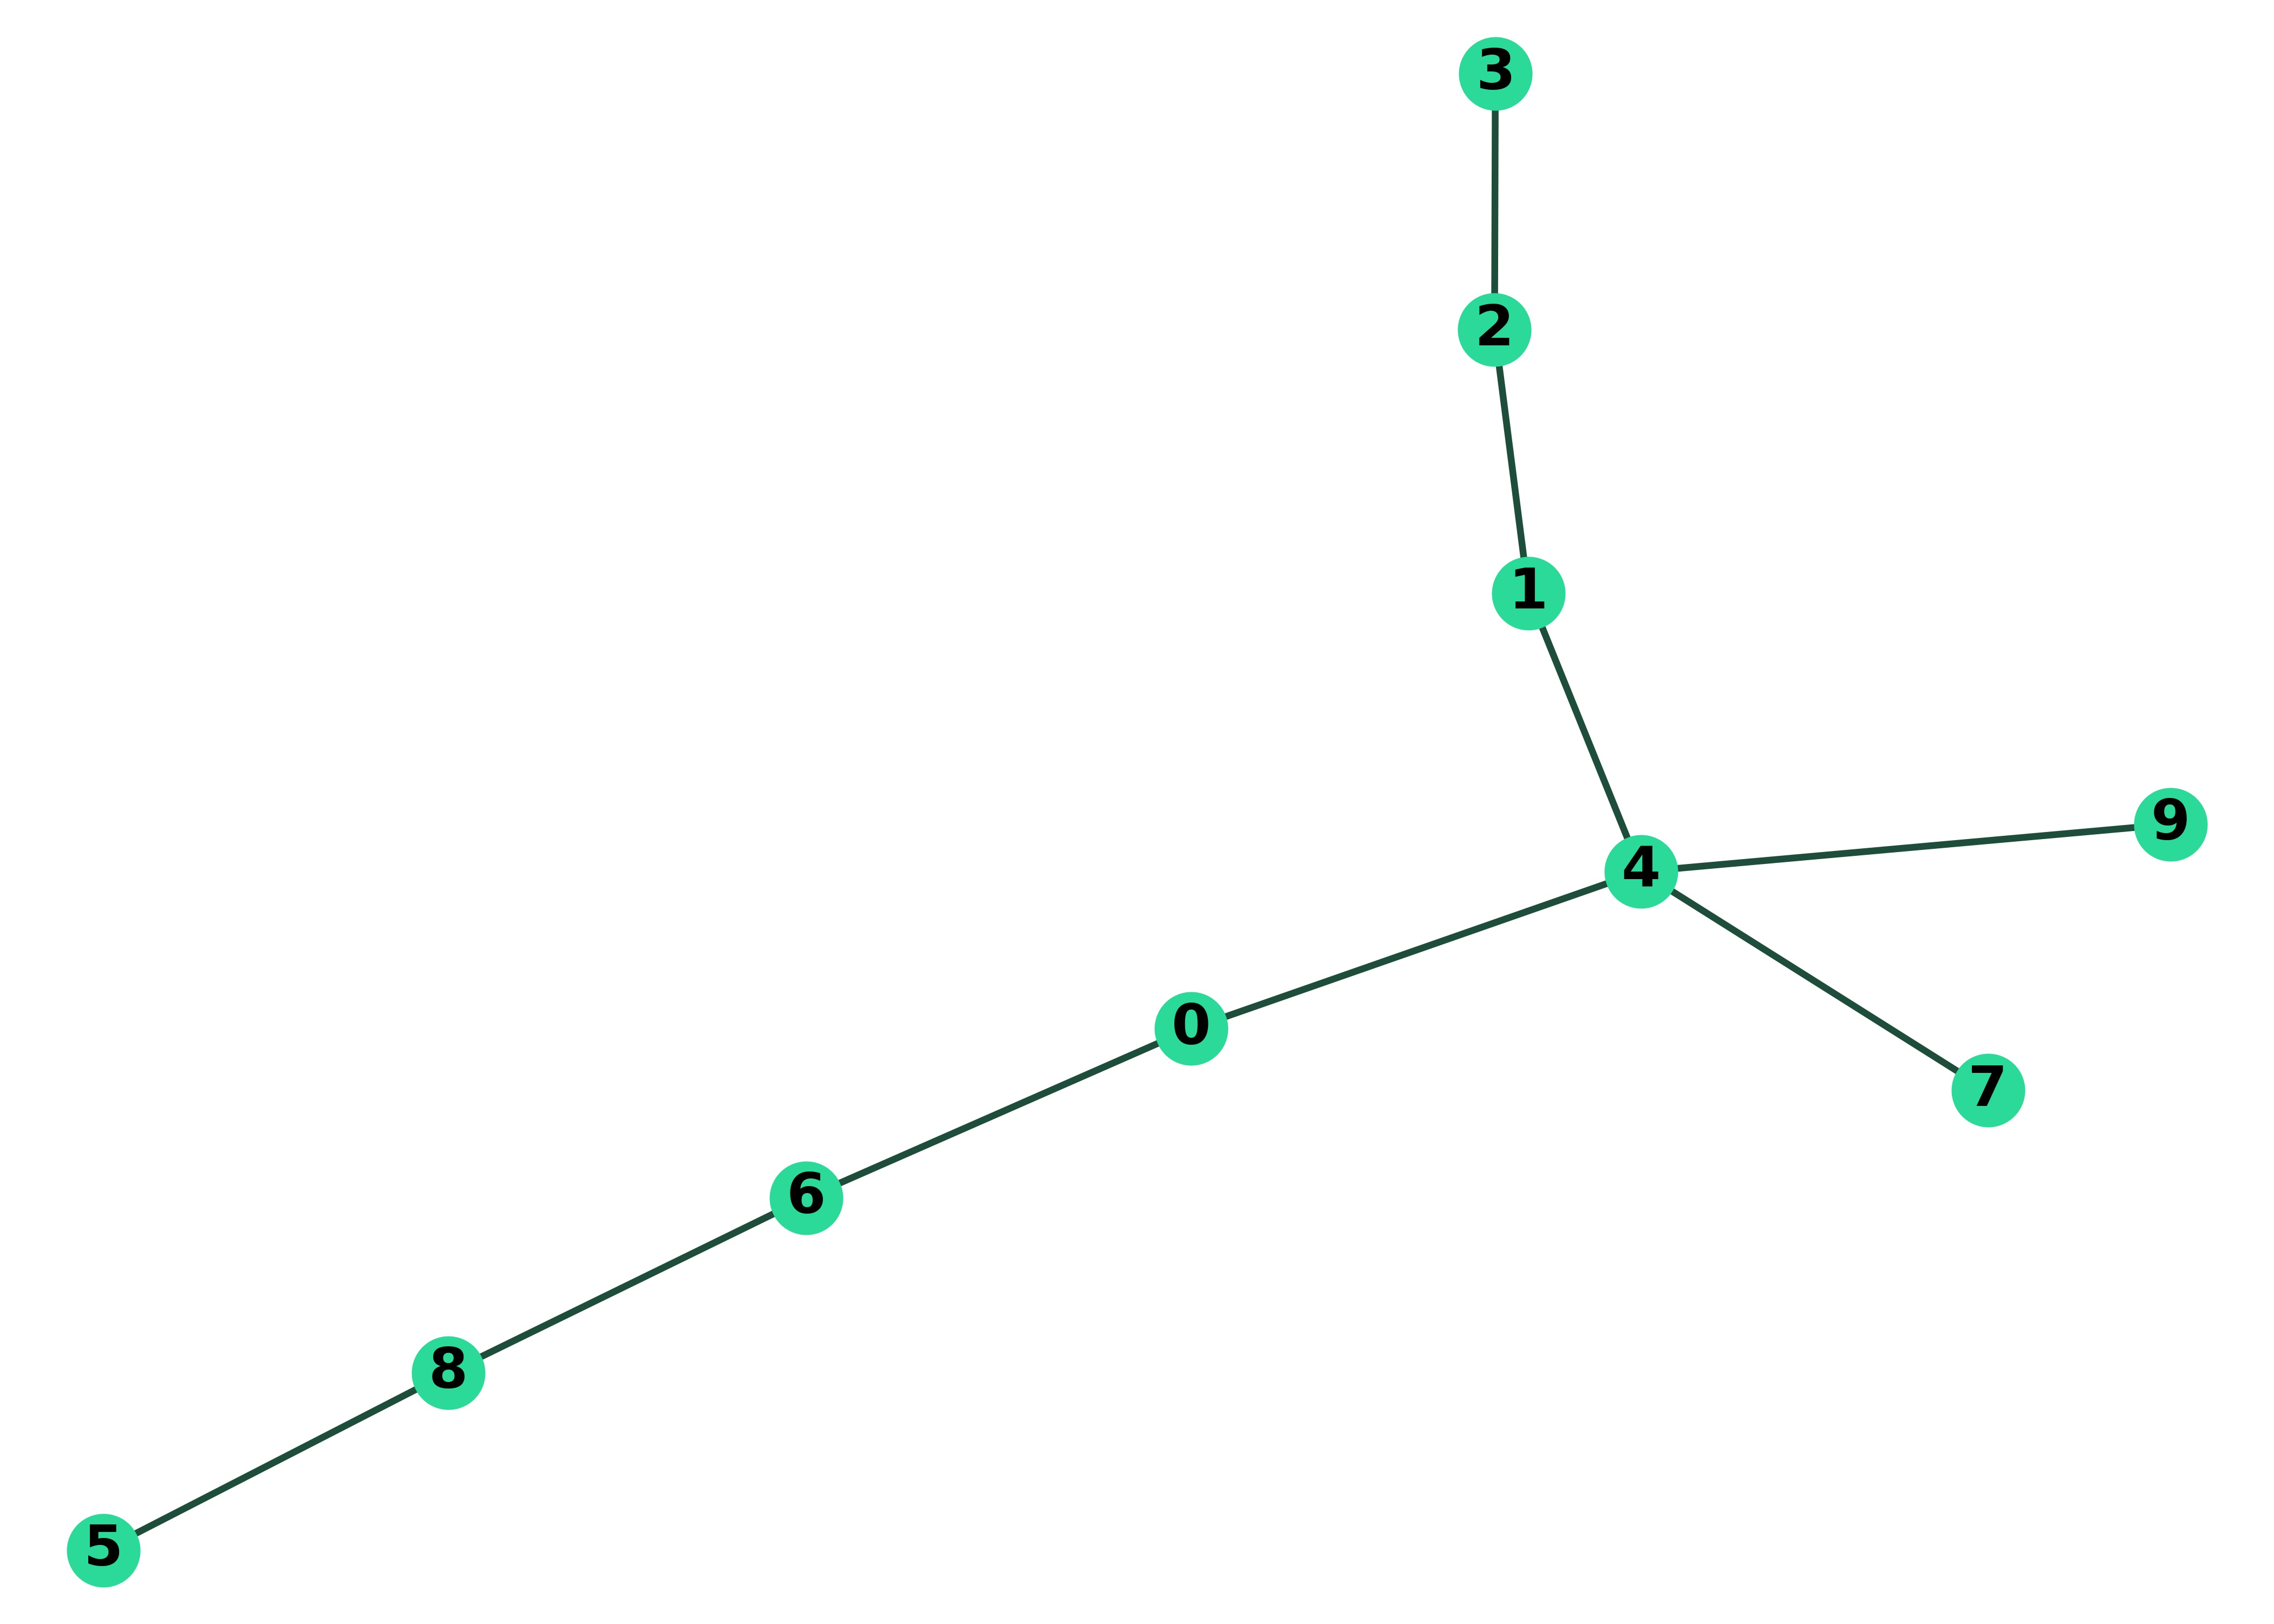
\includegraphics[width=.8\linewidth,valign=t]{assets/tree}
\end{column}

\begin{column}{.4\textwidth}
\textbf{Example: Tree}

\vspace{5pt}

A tree is a special type of graph where {\it any two vertices are connected by exactly one path.}
\end{column}

\end{columns}

\end{frame}

% -----------------

\begin{frame}{Examples of Graphs}

\begin{columns}

\begin{column}{.6\textwidth}
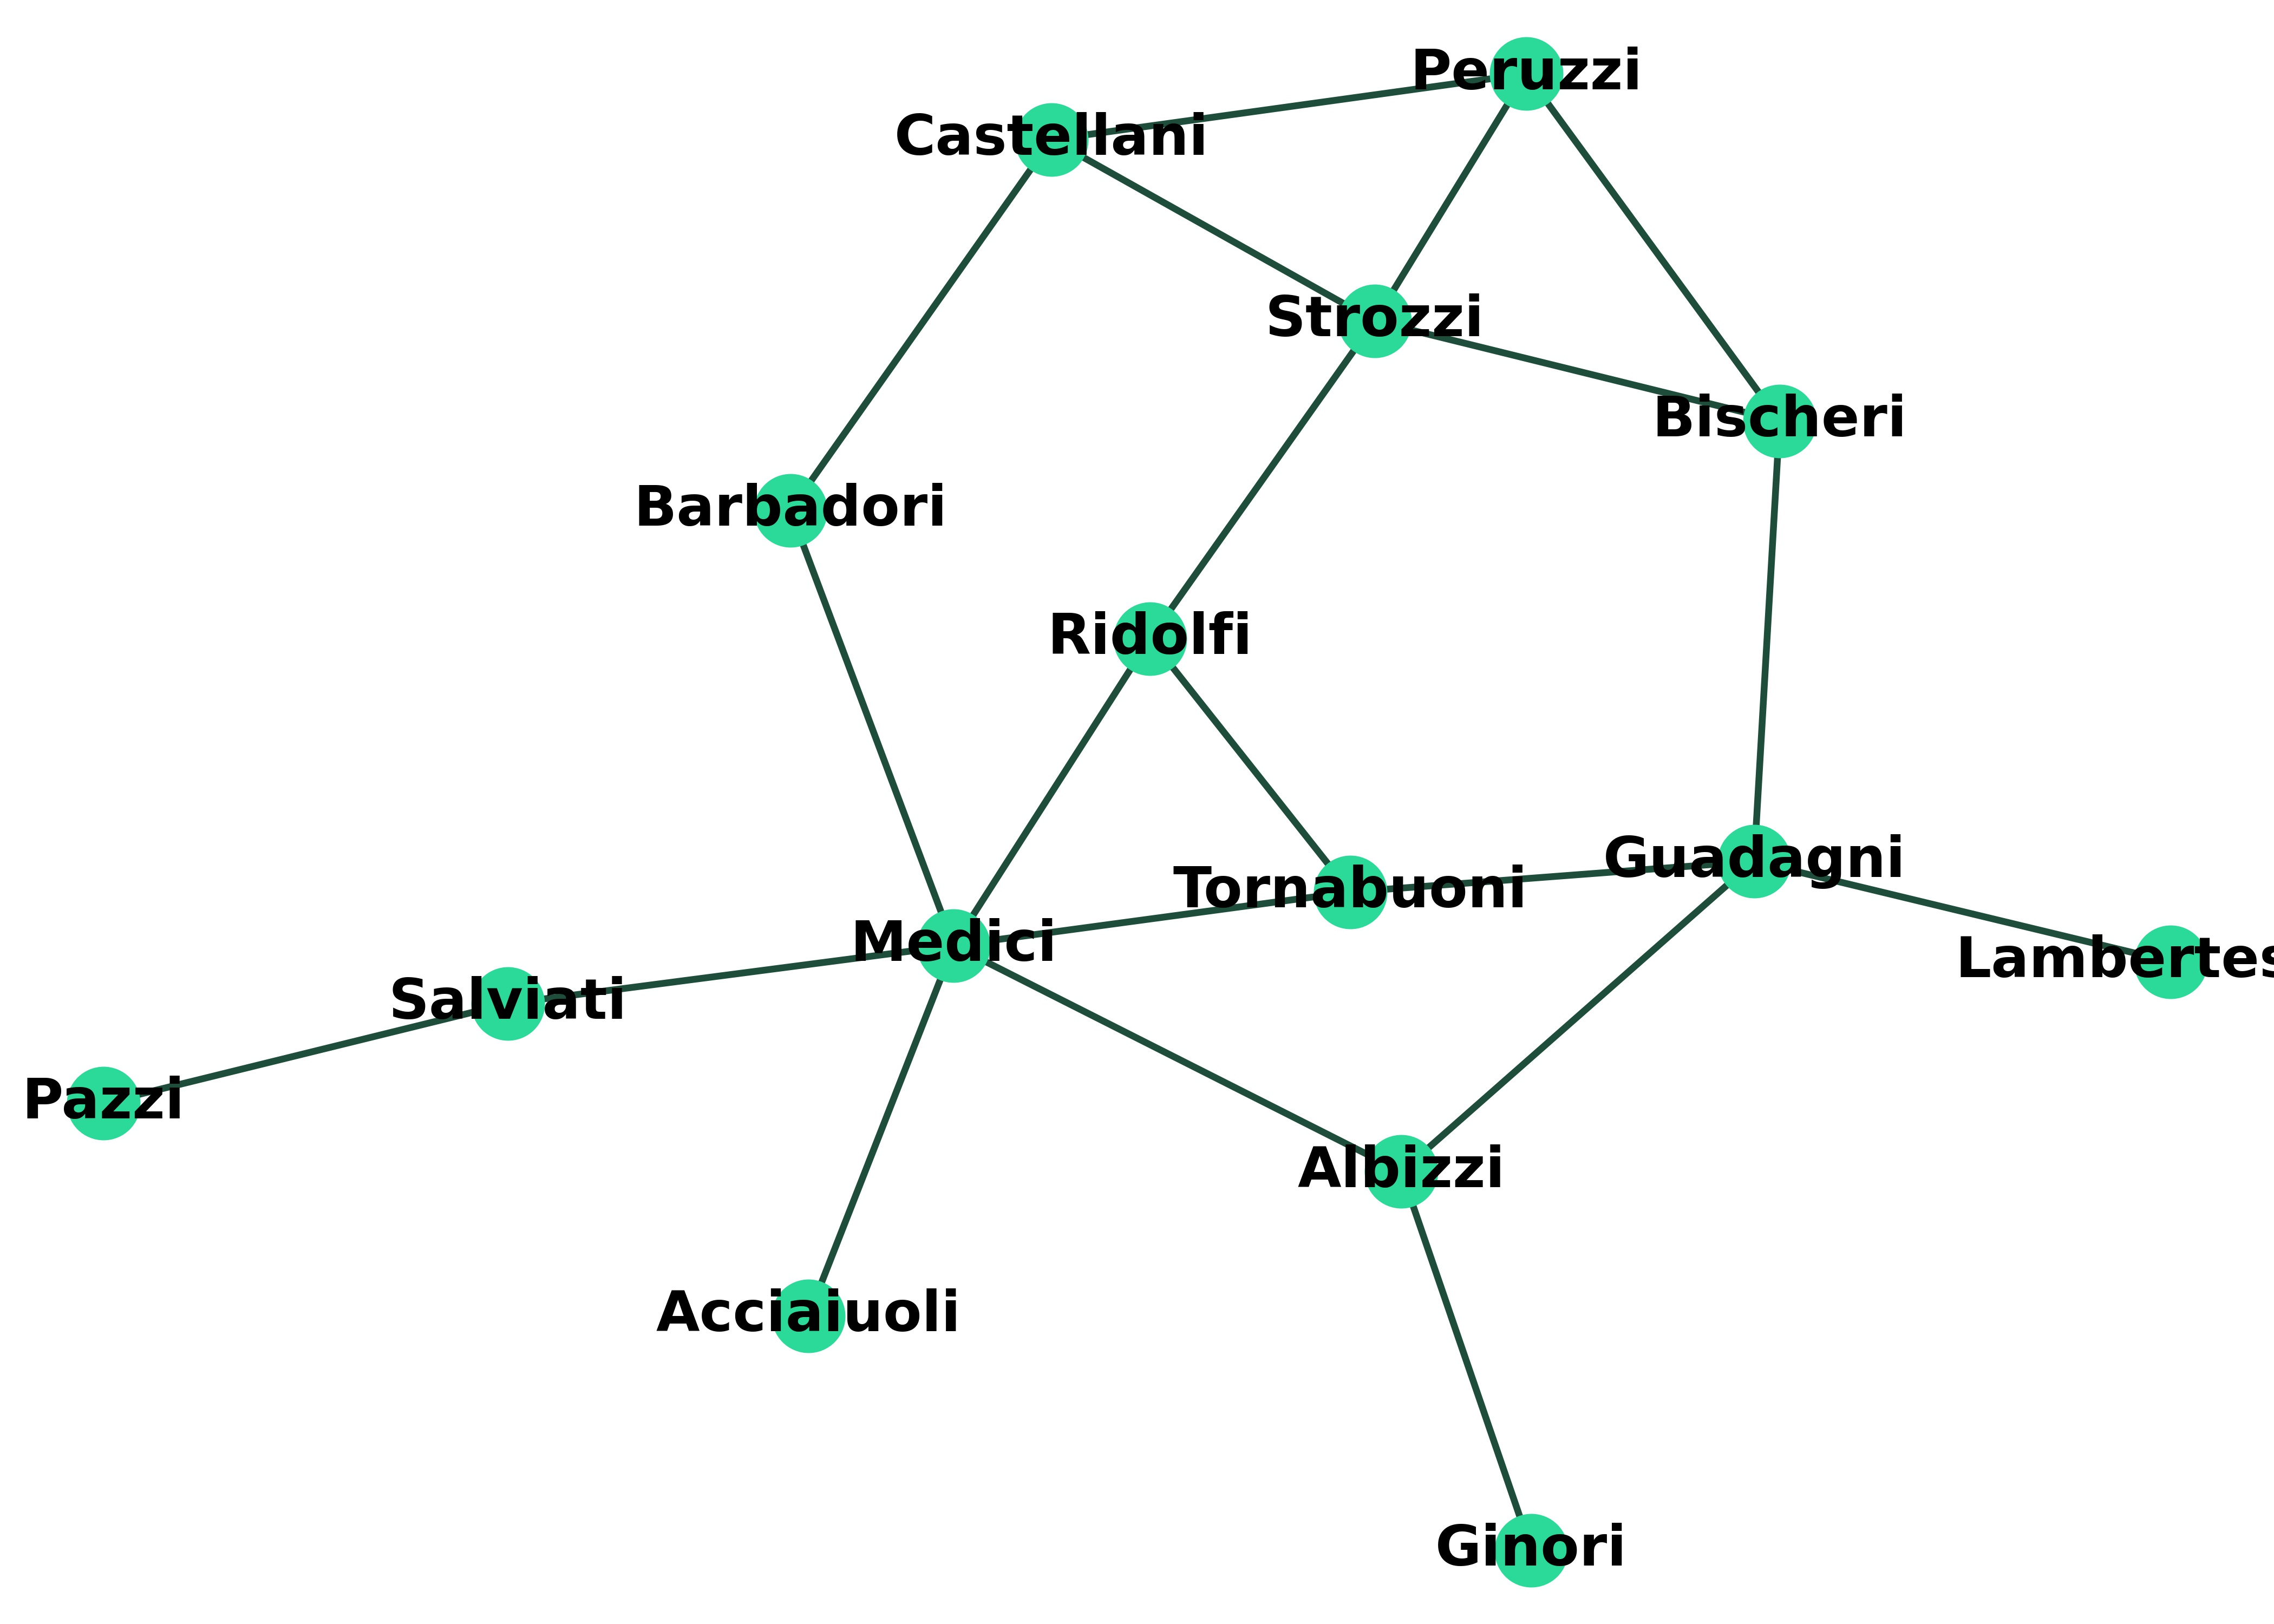
\includegraphics[width=.8\linewidth,valign=t]{assets/florentine}
\end{column}

\begin{column}{.4\textwidth}
\textbf{Example: Florentine Families Graph}
\vspace{5pt}

Depicts the marital alliances between Renaissance Florentine families \cite{padgett_1993}.

\end{column}

\end{columns}

\end{frame}

% -----------------------------------------------------------------------------
\subsection{Games on Graphs}

\begin{frame}{Using Graphs to Model Disease Spread}

\textbf{The Firefighter Problem ({\scshape Firefighter})} \cite{hartnell_1995} models an outbreak of fire with a firefighter strategically blocking its path.

\begin{itemize}
	\pause
	\item At $t=0$, a fire breaks out at some vertex in the graph.
	\pause
	\item Firefighter then `protects' some other vertex.
	\pause
	\item Fire spreads to any adjacent vertices neither protected nor burnt. 
	\pause
	\item Firefighter protects another vertex, the fire spreads again and so on.
\end{itemize}

\end{frame}

% -----------------

\begin{frame}{Example}
\centering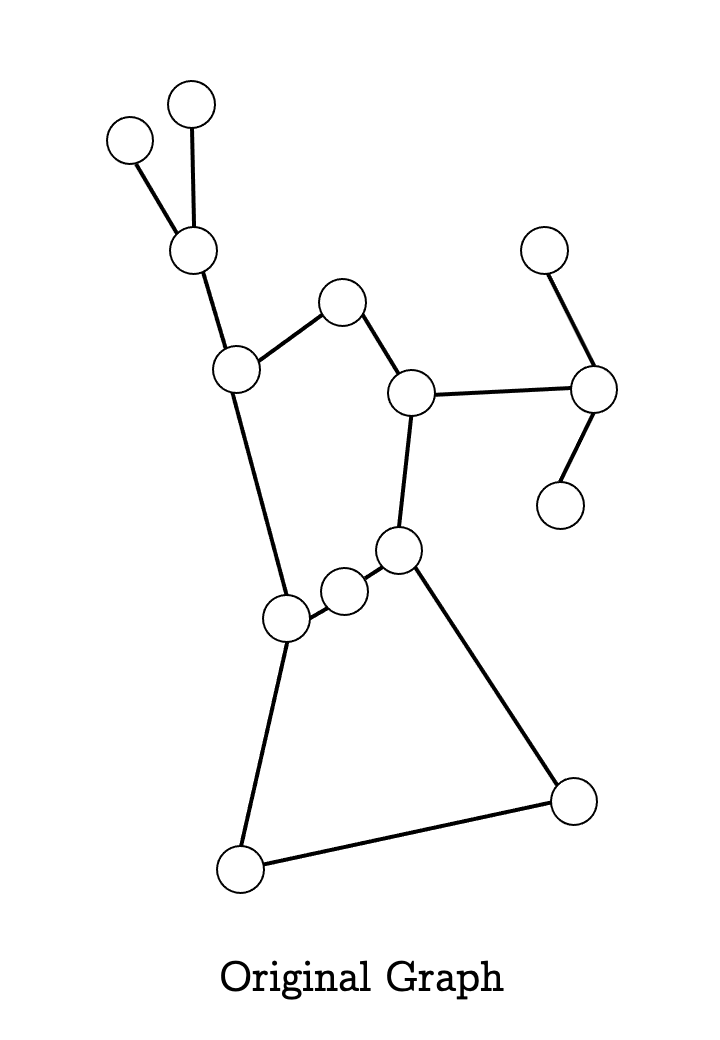
\includegraphics[height=0.8\textheight]{assets/eg-fire/0}
\end{frame}

\begin{frame}{Example}
\centering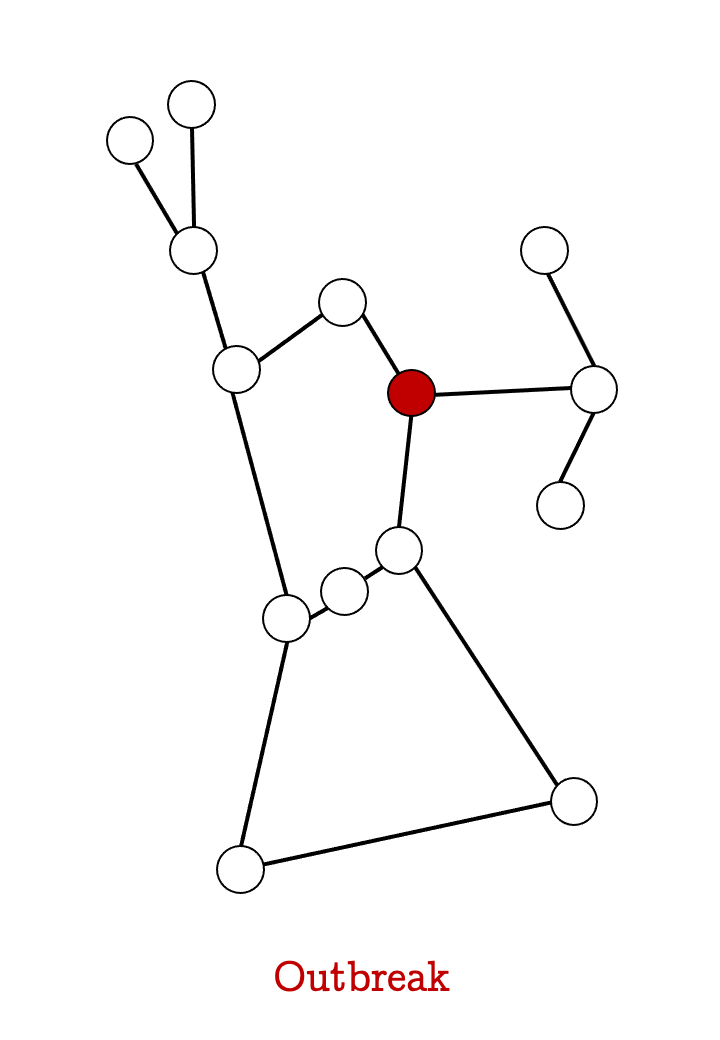
\includegraphics[height=0.8\textheight]{assets/eg-fire/1}
\end{frame}

\begin{frame}{Example}
\centering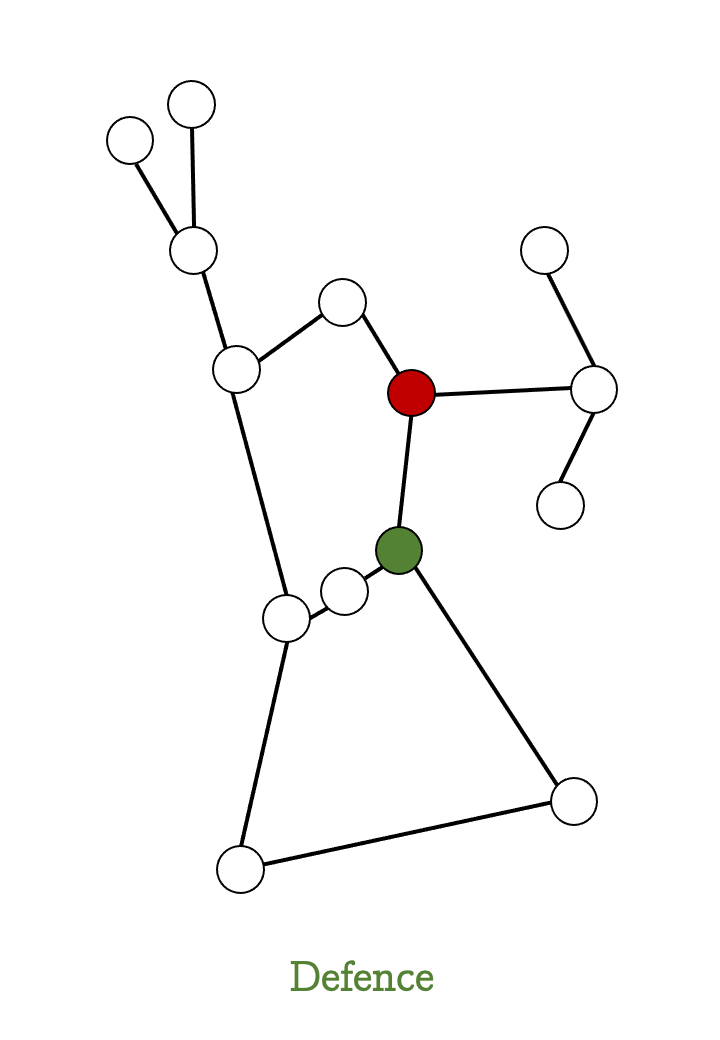
\includegraphics[height=0.8\textheight]{assets/eg-fire/2}
\end{frame}

\begin{frame}{Example}
\centering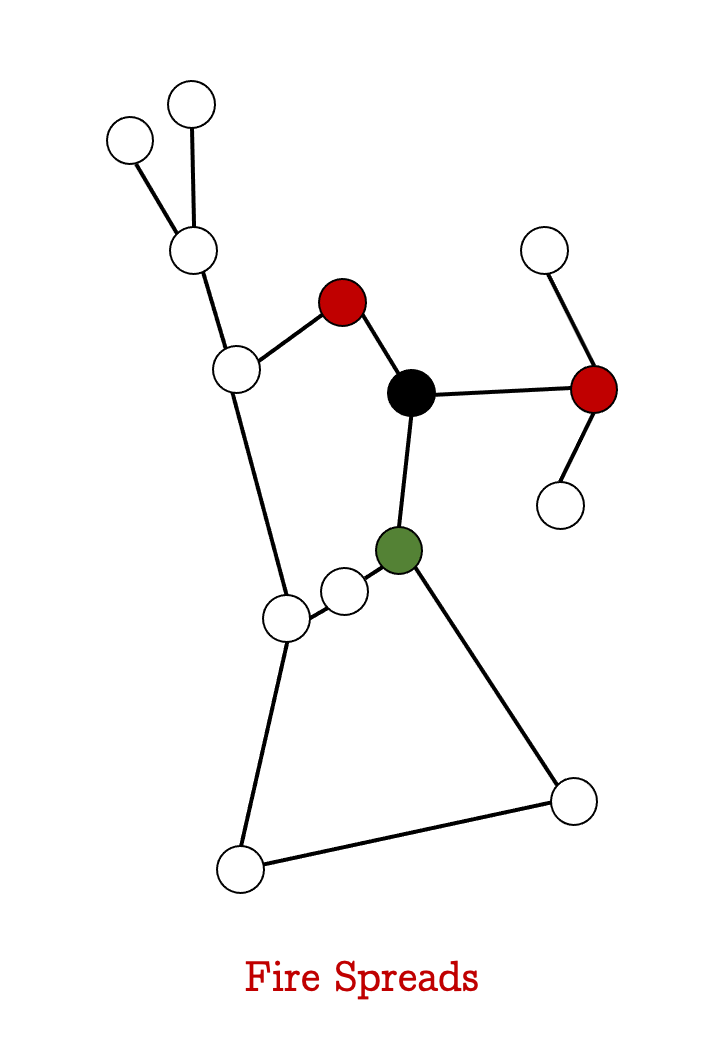
\includegraphics[height=0.8\textheight]{assets/eg-fire/3}
\end{frame}

\begin{frame}{Example}
\centering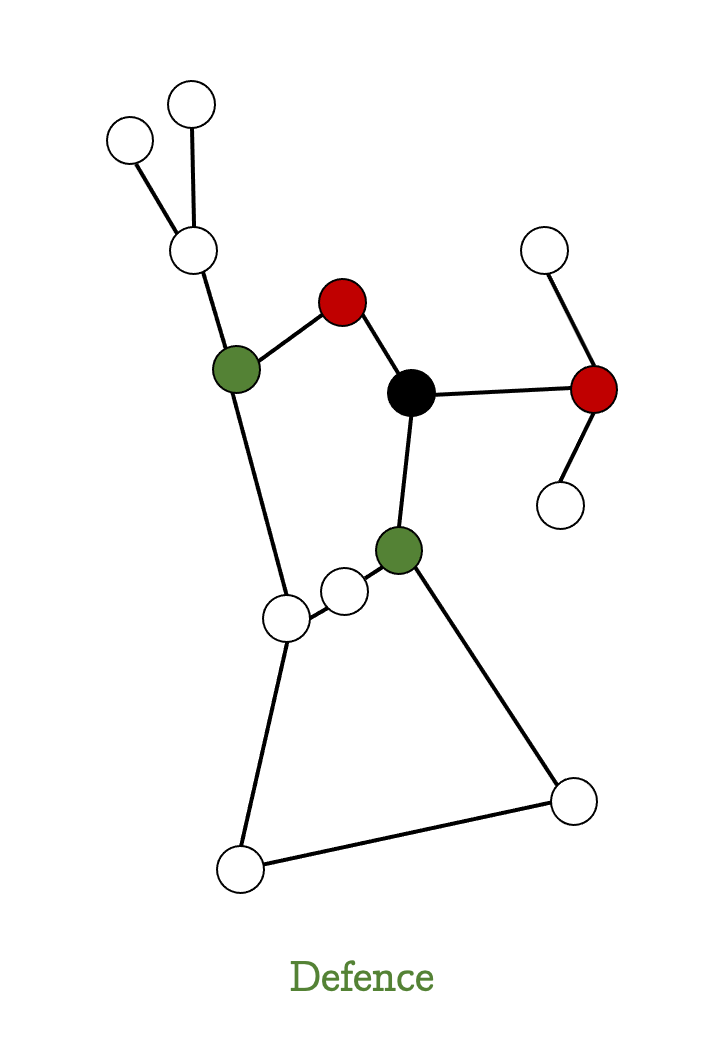
\includegraphics[height=0.8\textheight]{assets/eg-fire/4}
\end{frame}

\begin{frame}{Example}
\centering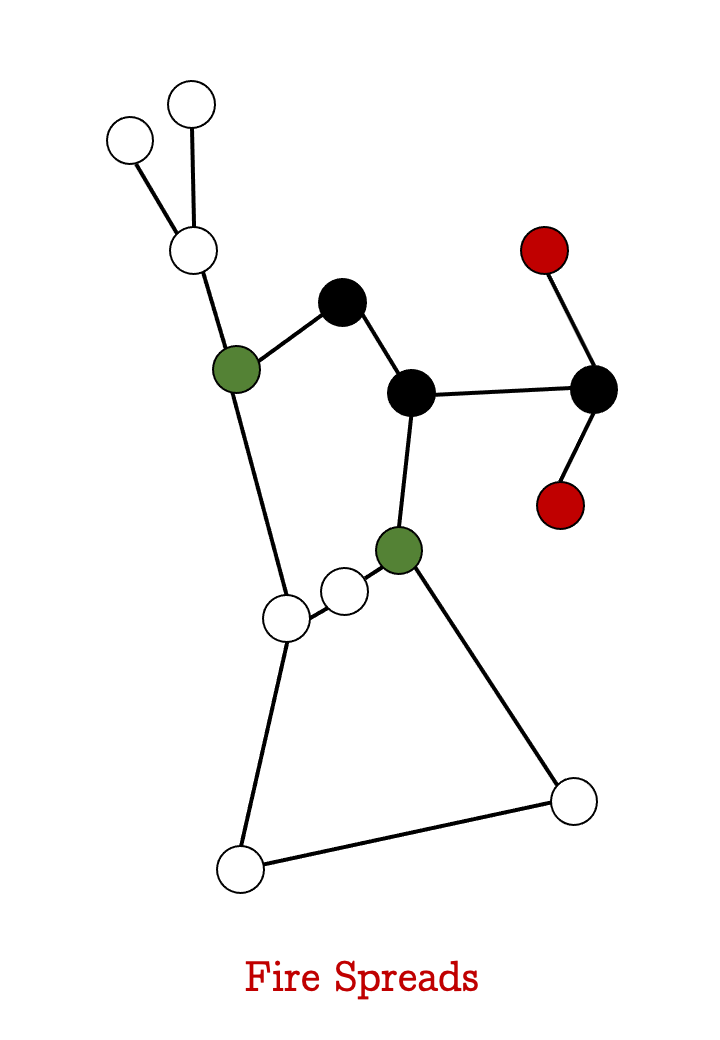
\includegraphics[height=0.8\textheight]{assets/eg-fire/5}
\end{frame}

\begin{frame}{Example}
\centering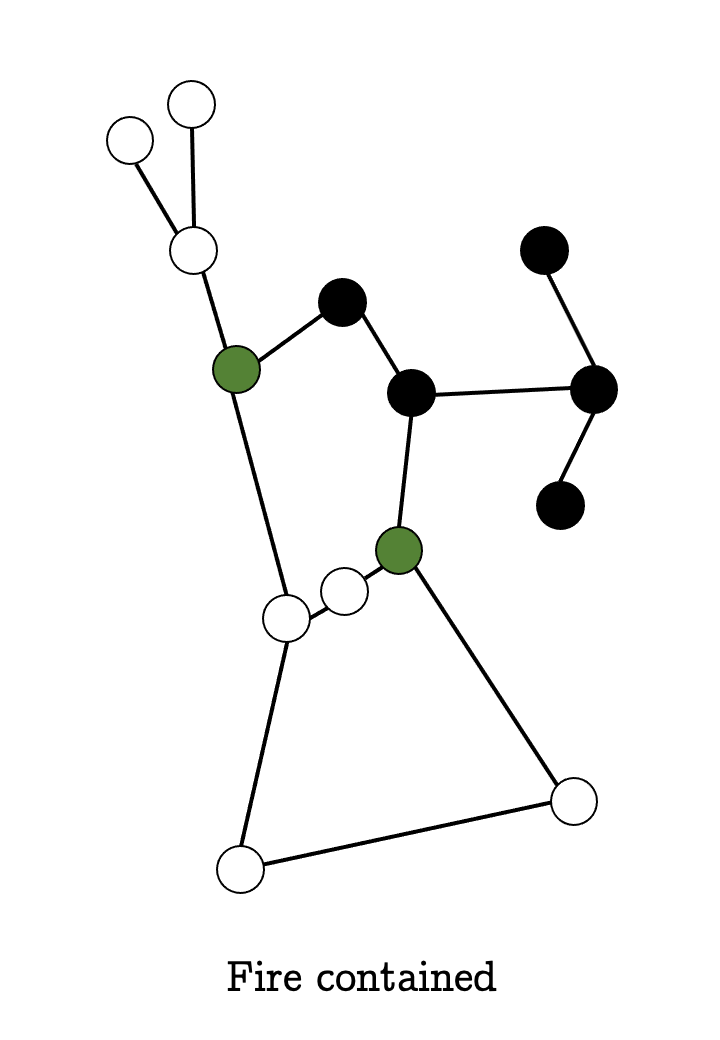
\includegraphics[height=0.8\textheight]{assets/eg-fire/6}
\end{frame}

% -----------------

\begin{frame}{Firefighter as a Model for Disease Spread}

Benefits:
\begin{itemize}
	\pause
	\item Previous work means lots of results we can use.
	\pause
	\item We can change graphs to suit context - e.g. small world, preferential attachment, particular density.
\end{itemize}
\pause
Limitations:
\begin{itemize}
	\pause
	\item Fairly rudimentary model for disease spread but already NP-hard.
	\pause
	\item Defence and infection are discrete but epidemic propagation is a stochastic process.
	\pause
	\item Only interventions in halting disease spread are {\it external}, no way for individuals to avoid contraction personally.
\end{itemize}
	
\end{frame}

% =============================================================================
\section{Extending existing graph models to account for agency}

% -----------------------------------------------------------------------------
\begin{frame}
  \frametitle{Outline}
  \tableofcontents[currentsection]
\end{frame}
% -----------------------------------------------------------------------------
\subsection{Attributes of Agency}
\begin{frame}{Attributes of Agency}

If each vertex in the graph represents an individual agent, we can start to assign agency-related attributes. We are particularly interested in each agent's {\it internal inclination towards protection}. In context, this might involve:
\begin{itemize}
	\pause
	\item Wearing PPE correctly
	\pause
	\item Hand hygiene
	\pause
	\item Strict physical distancing
\end{itemize}

\end{frame}

\begin{frame}
\centering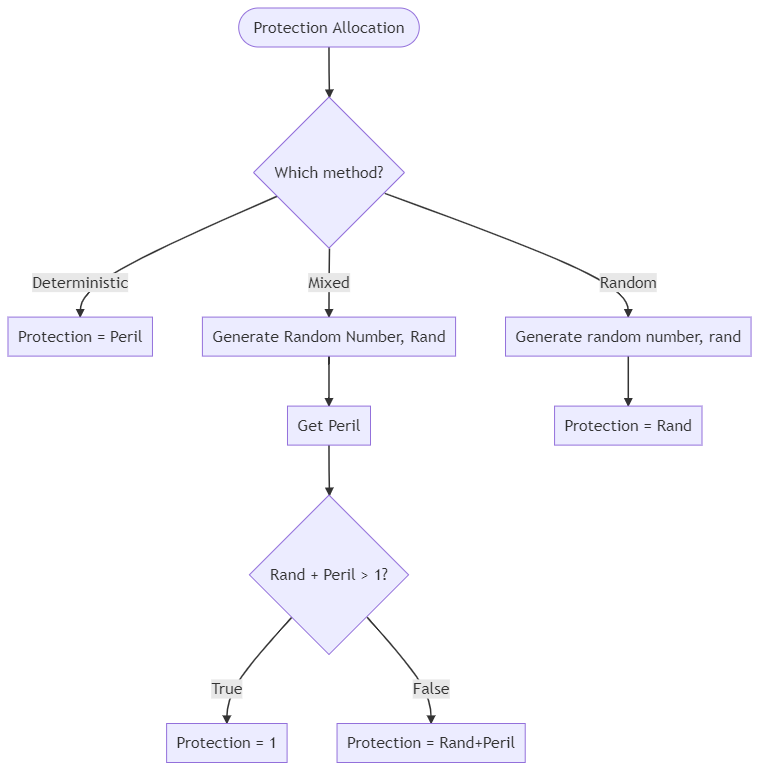
\includegraphics[height=.9\textheight]{assets/flowcharts/protection}
\end{frame}


% -----------------------------------------------------------------------------
\begin{frame}{Defence Strategies}

What do these amendments mean for how the game is played? In the usual formulation, general rule of thumb: {\it for sparse graphs, defend based on proximity to fire (breaking ties on degree); for dense graphs, defend based on degree (breaking ties on proximity)}. \pause

\vspace{5pt}

However, in our adjusted formulation we have more candidates for defence strategies. One such novel strategy is to defend based on highest agent protection rating.

\end{frame}

% -----------------------------------------------------------------------------
\subsection{Protection Rating Allocation and Defence Strategies}

\begin{frame}
\centering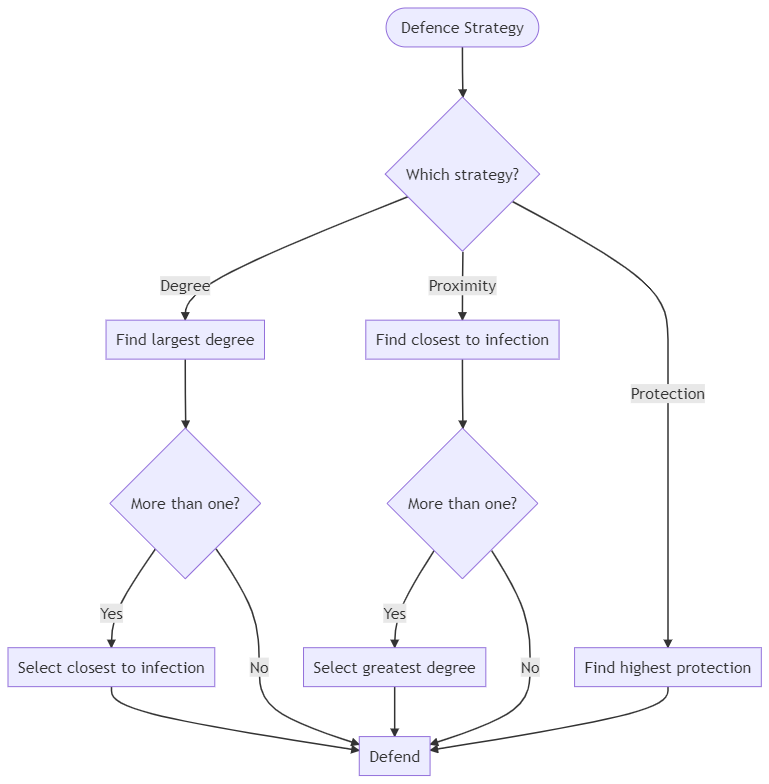
\includegraphics[height=.9\textheight]{assets/flowcharts/defence}
\end{frame}

% -----------------

\begin{frame}{Deterministic Protection}
\centering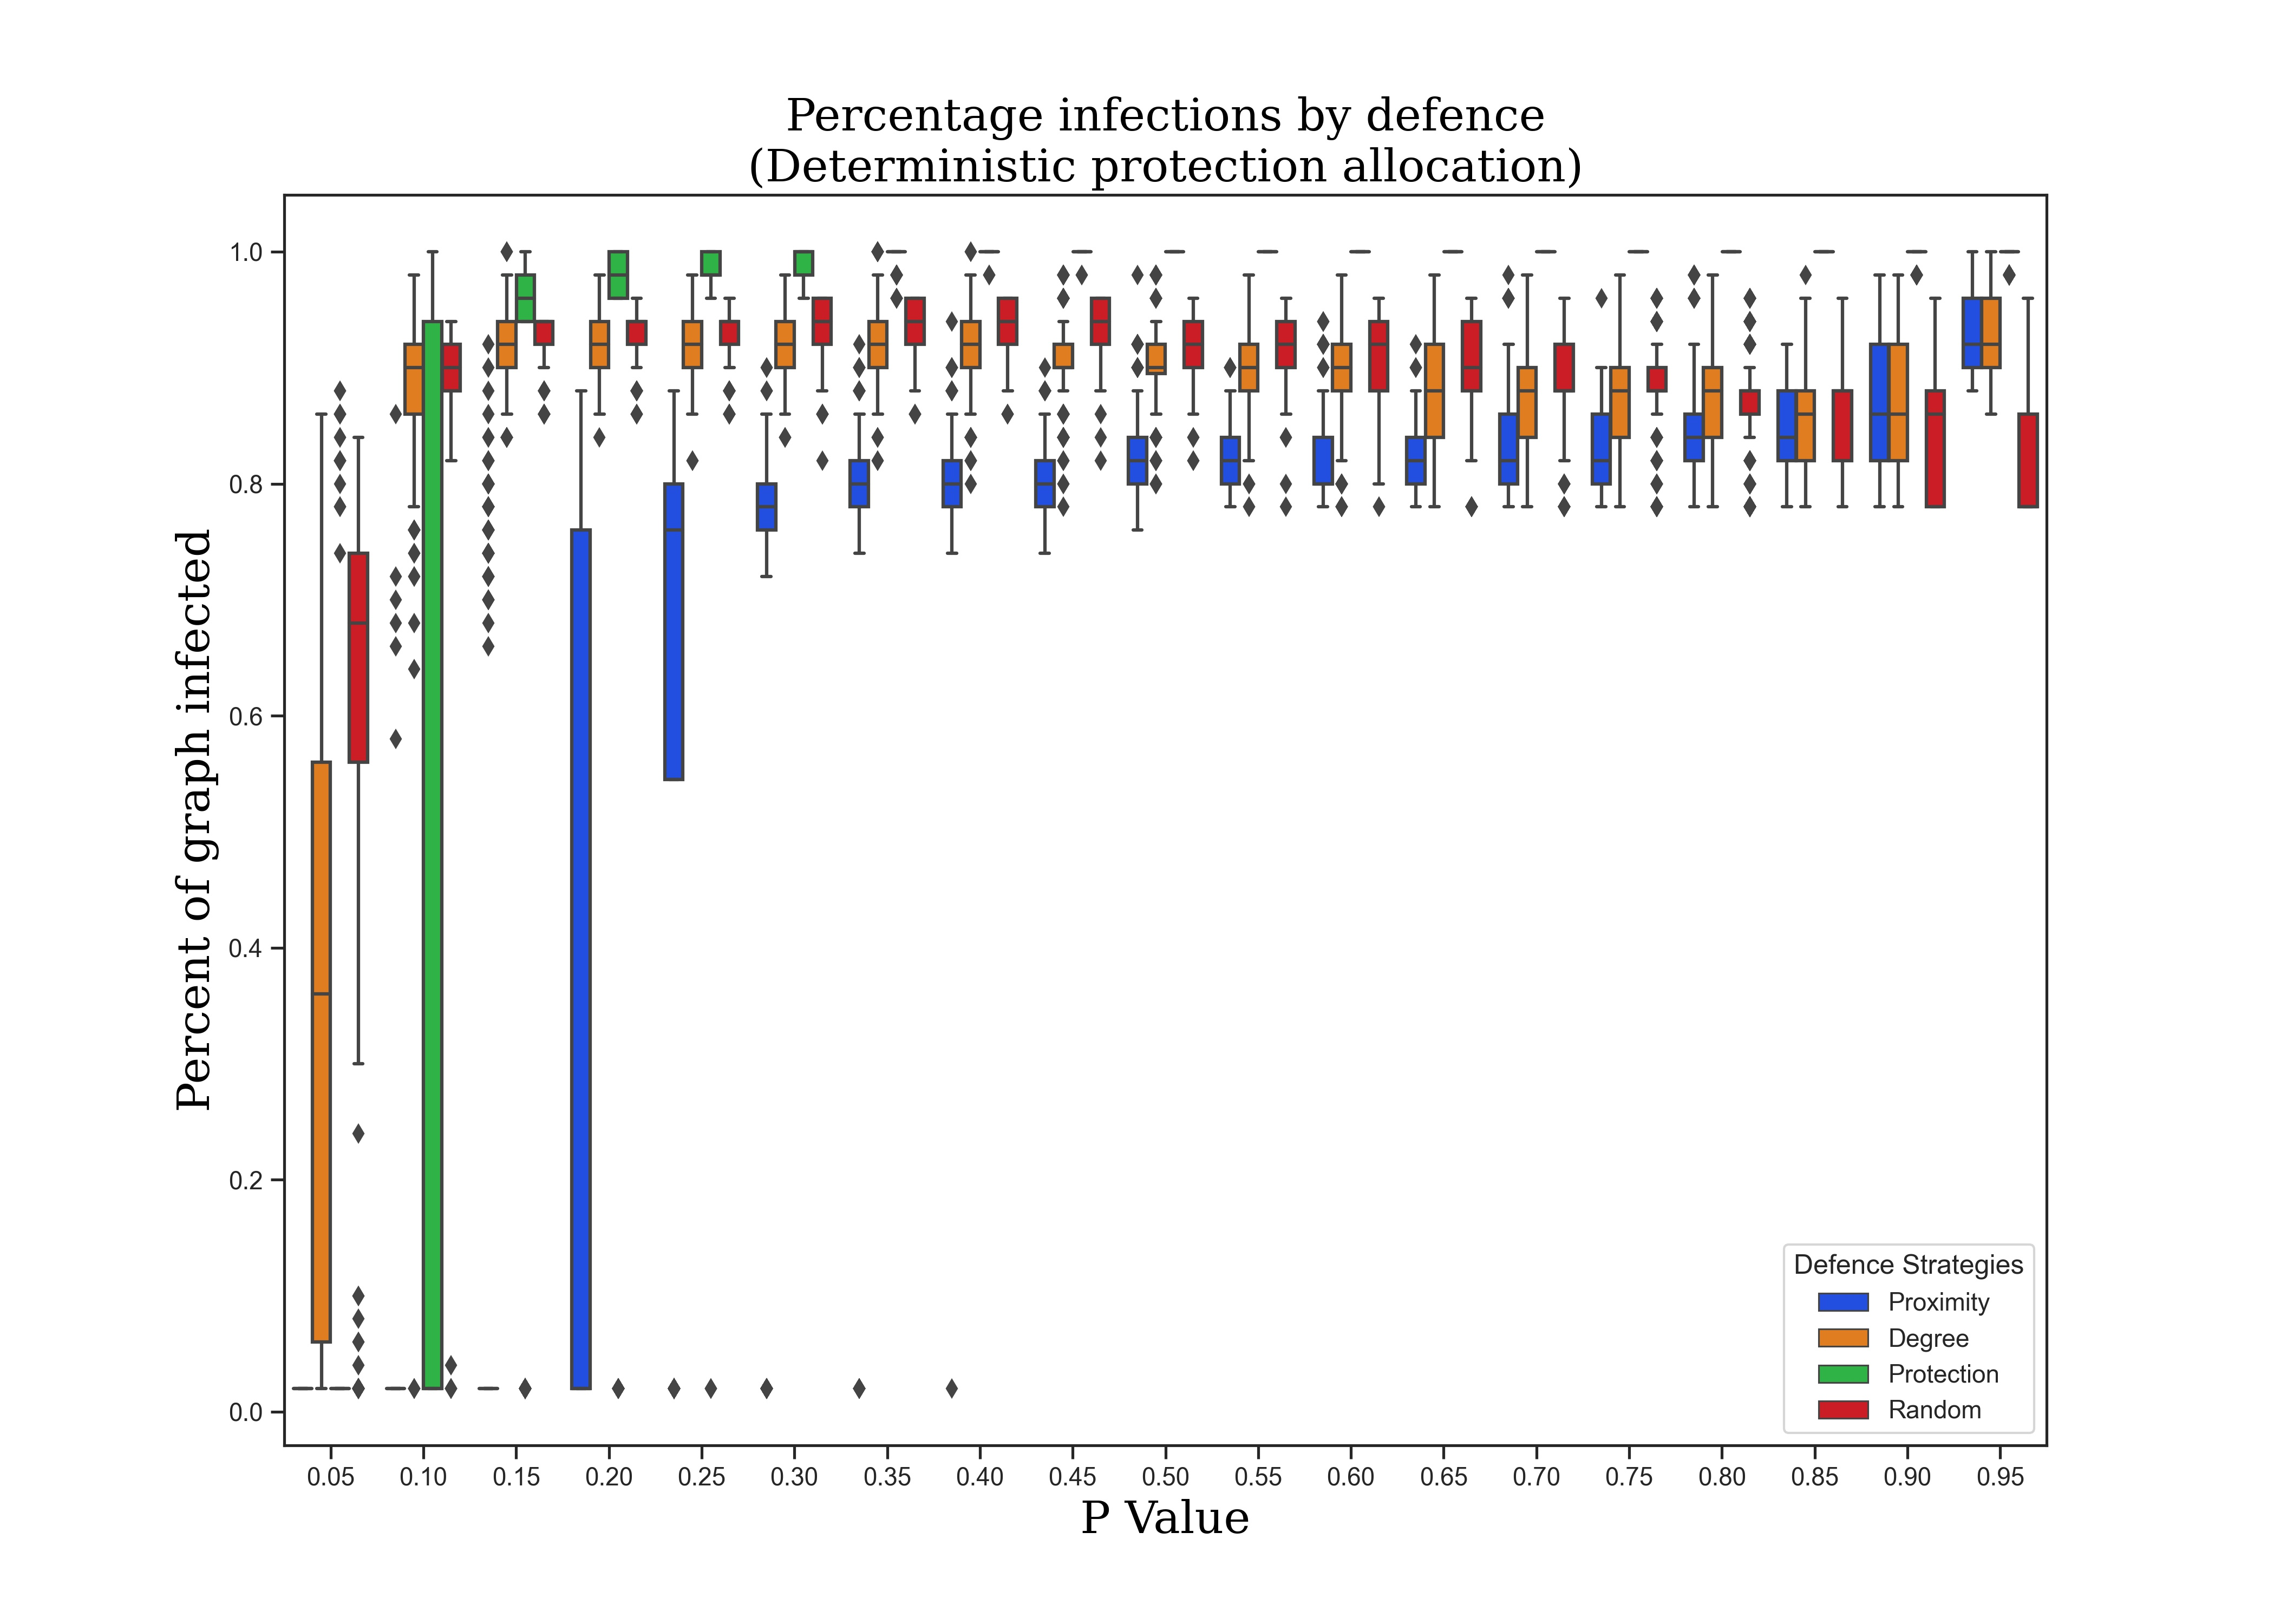
\includegraphics[height=0.85\textheight]{assets/charts/percent_infected/Deterministic.jpg}
\end{frame}

% -----------------
%
%\begin{frame}{Deterministic Protection}
%\centering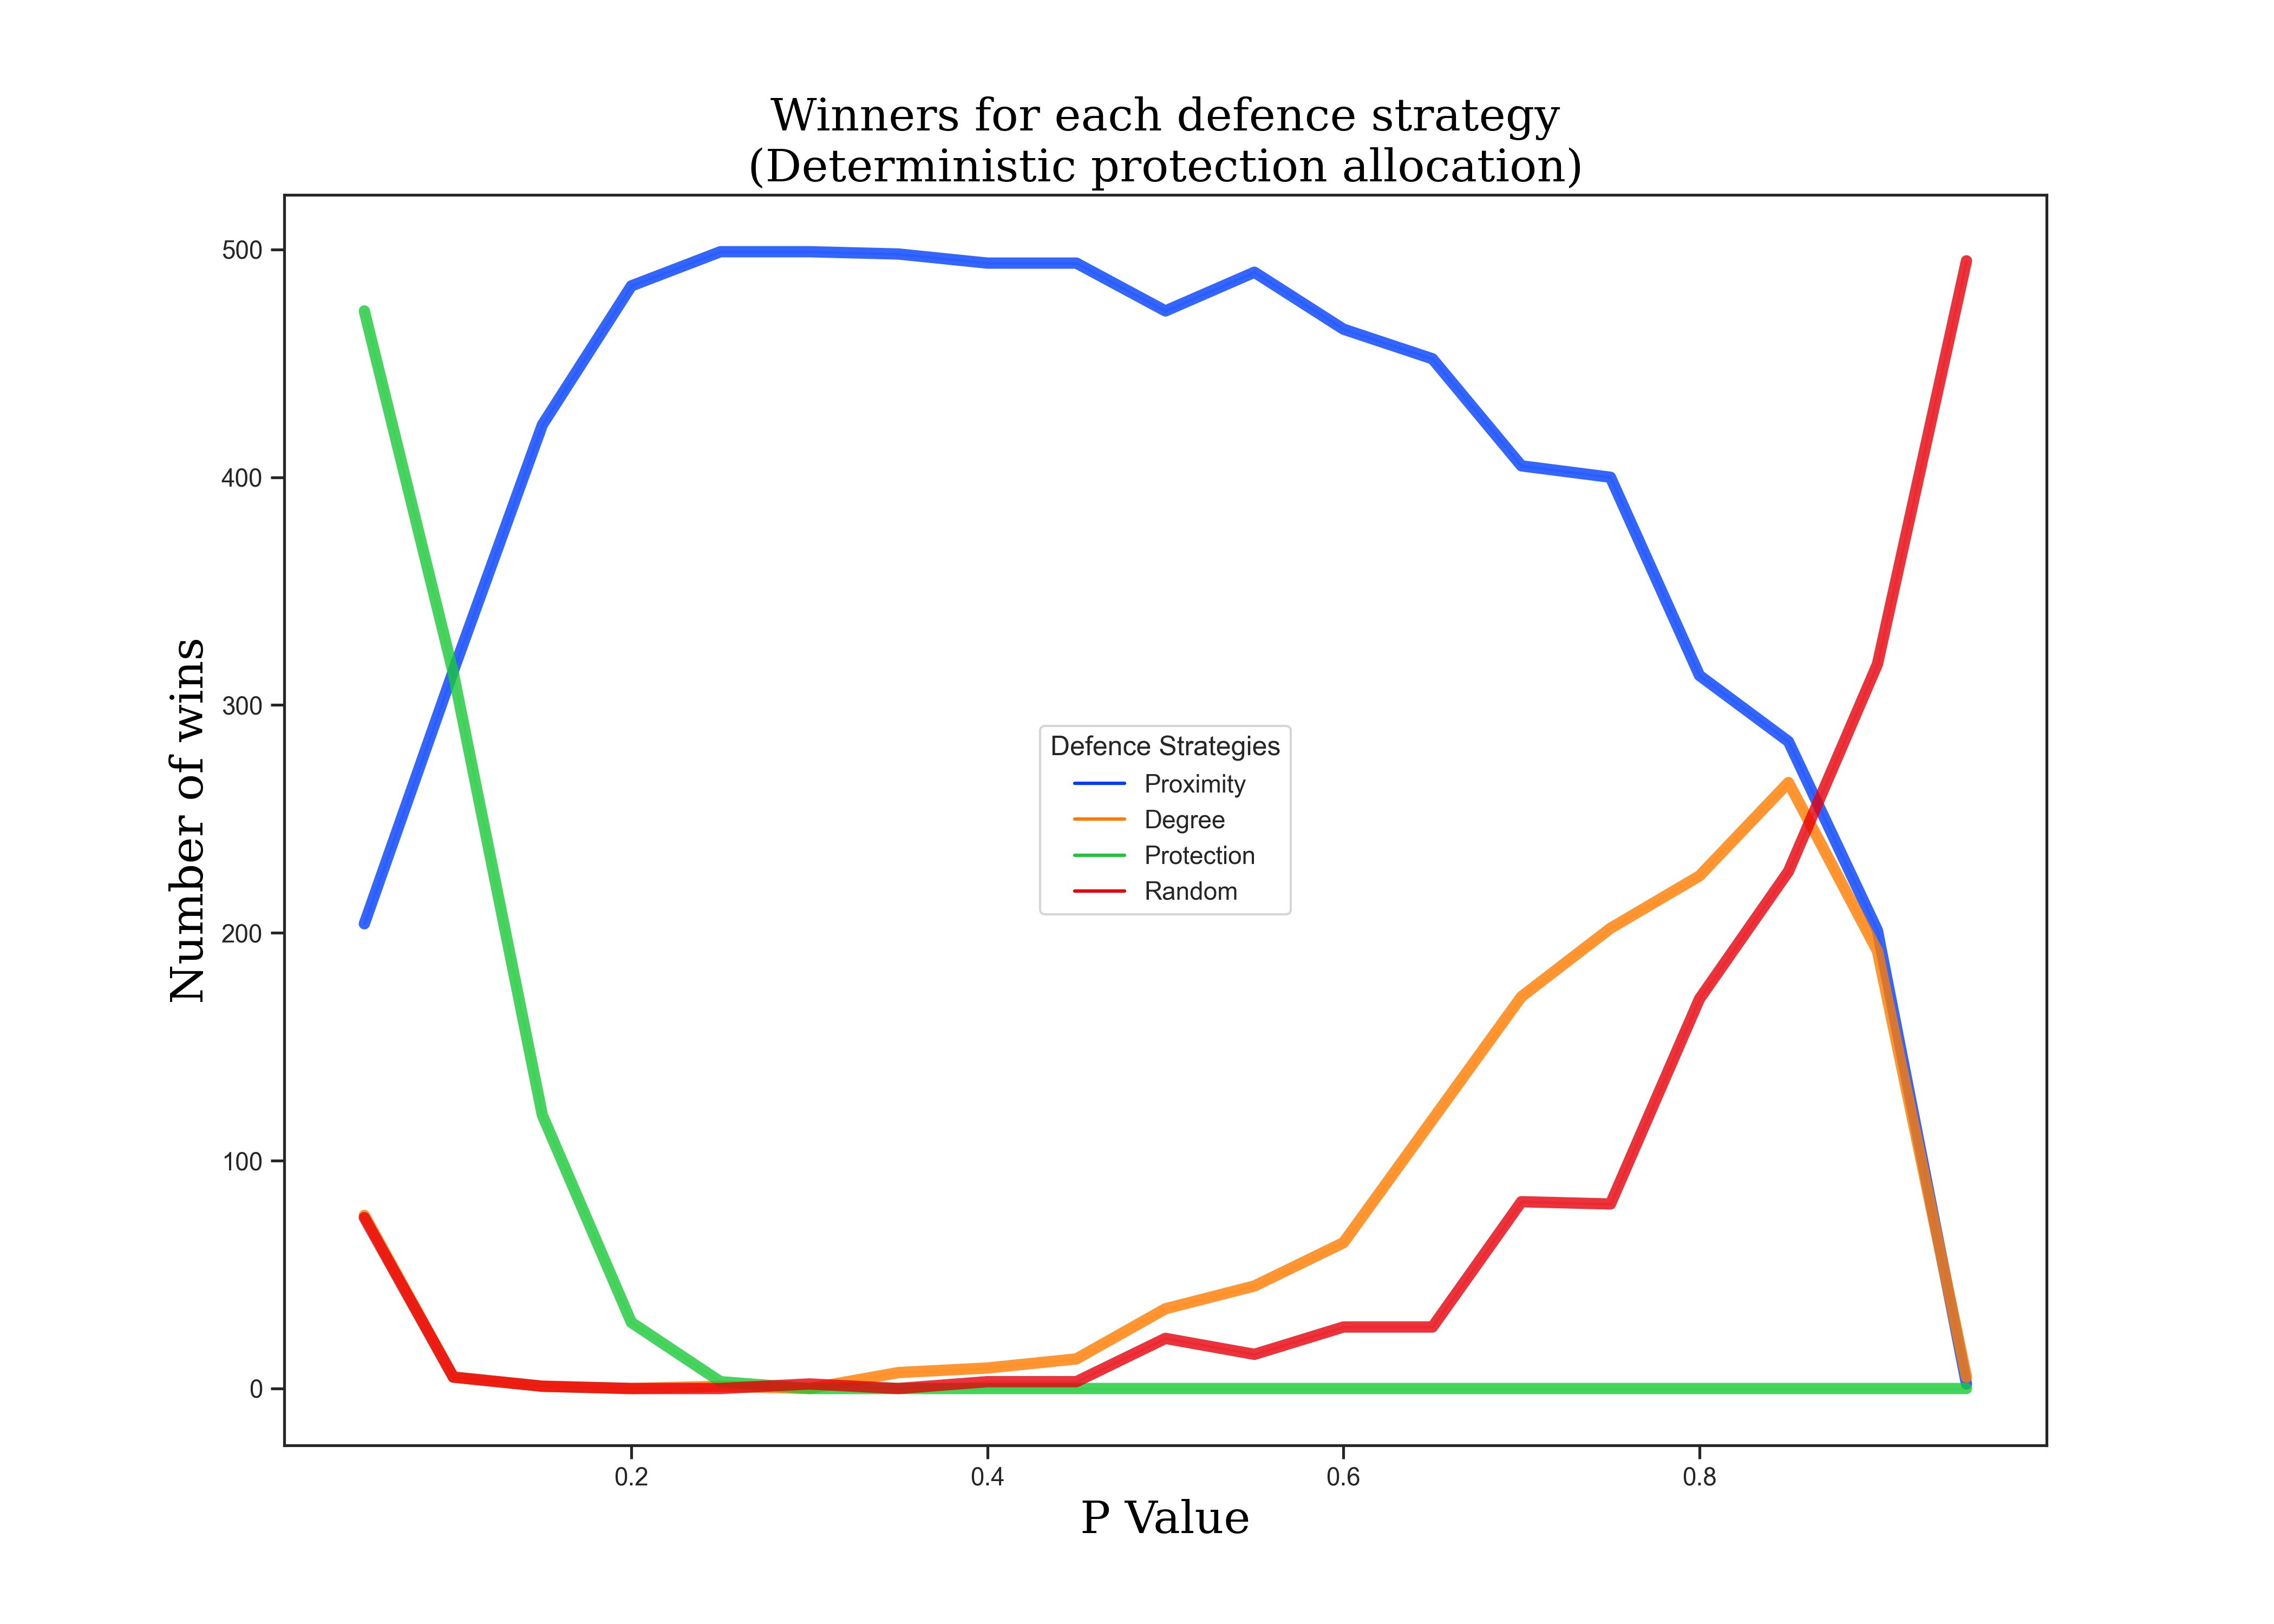
\includegraphics[height=0.8\textheight]{assets/charts/winners/Deterministic.jpg}
%\end{frame}

% -----------------

\begin{frame}{Mixed Protection}
\centering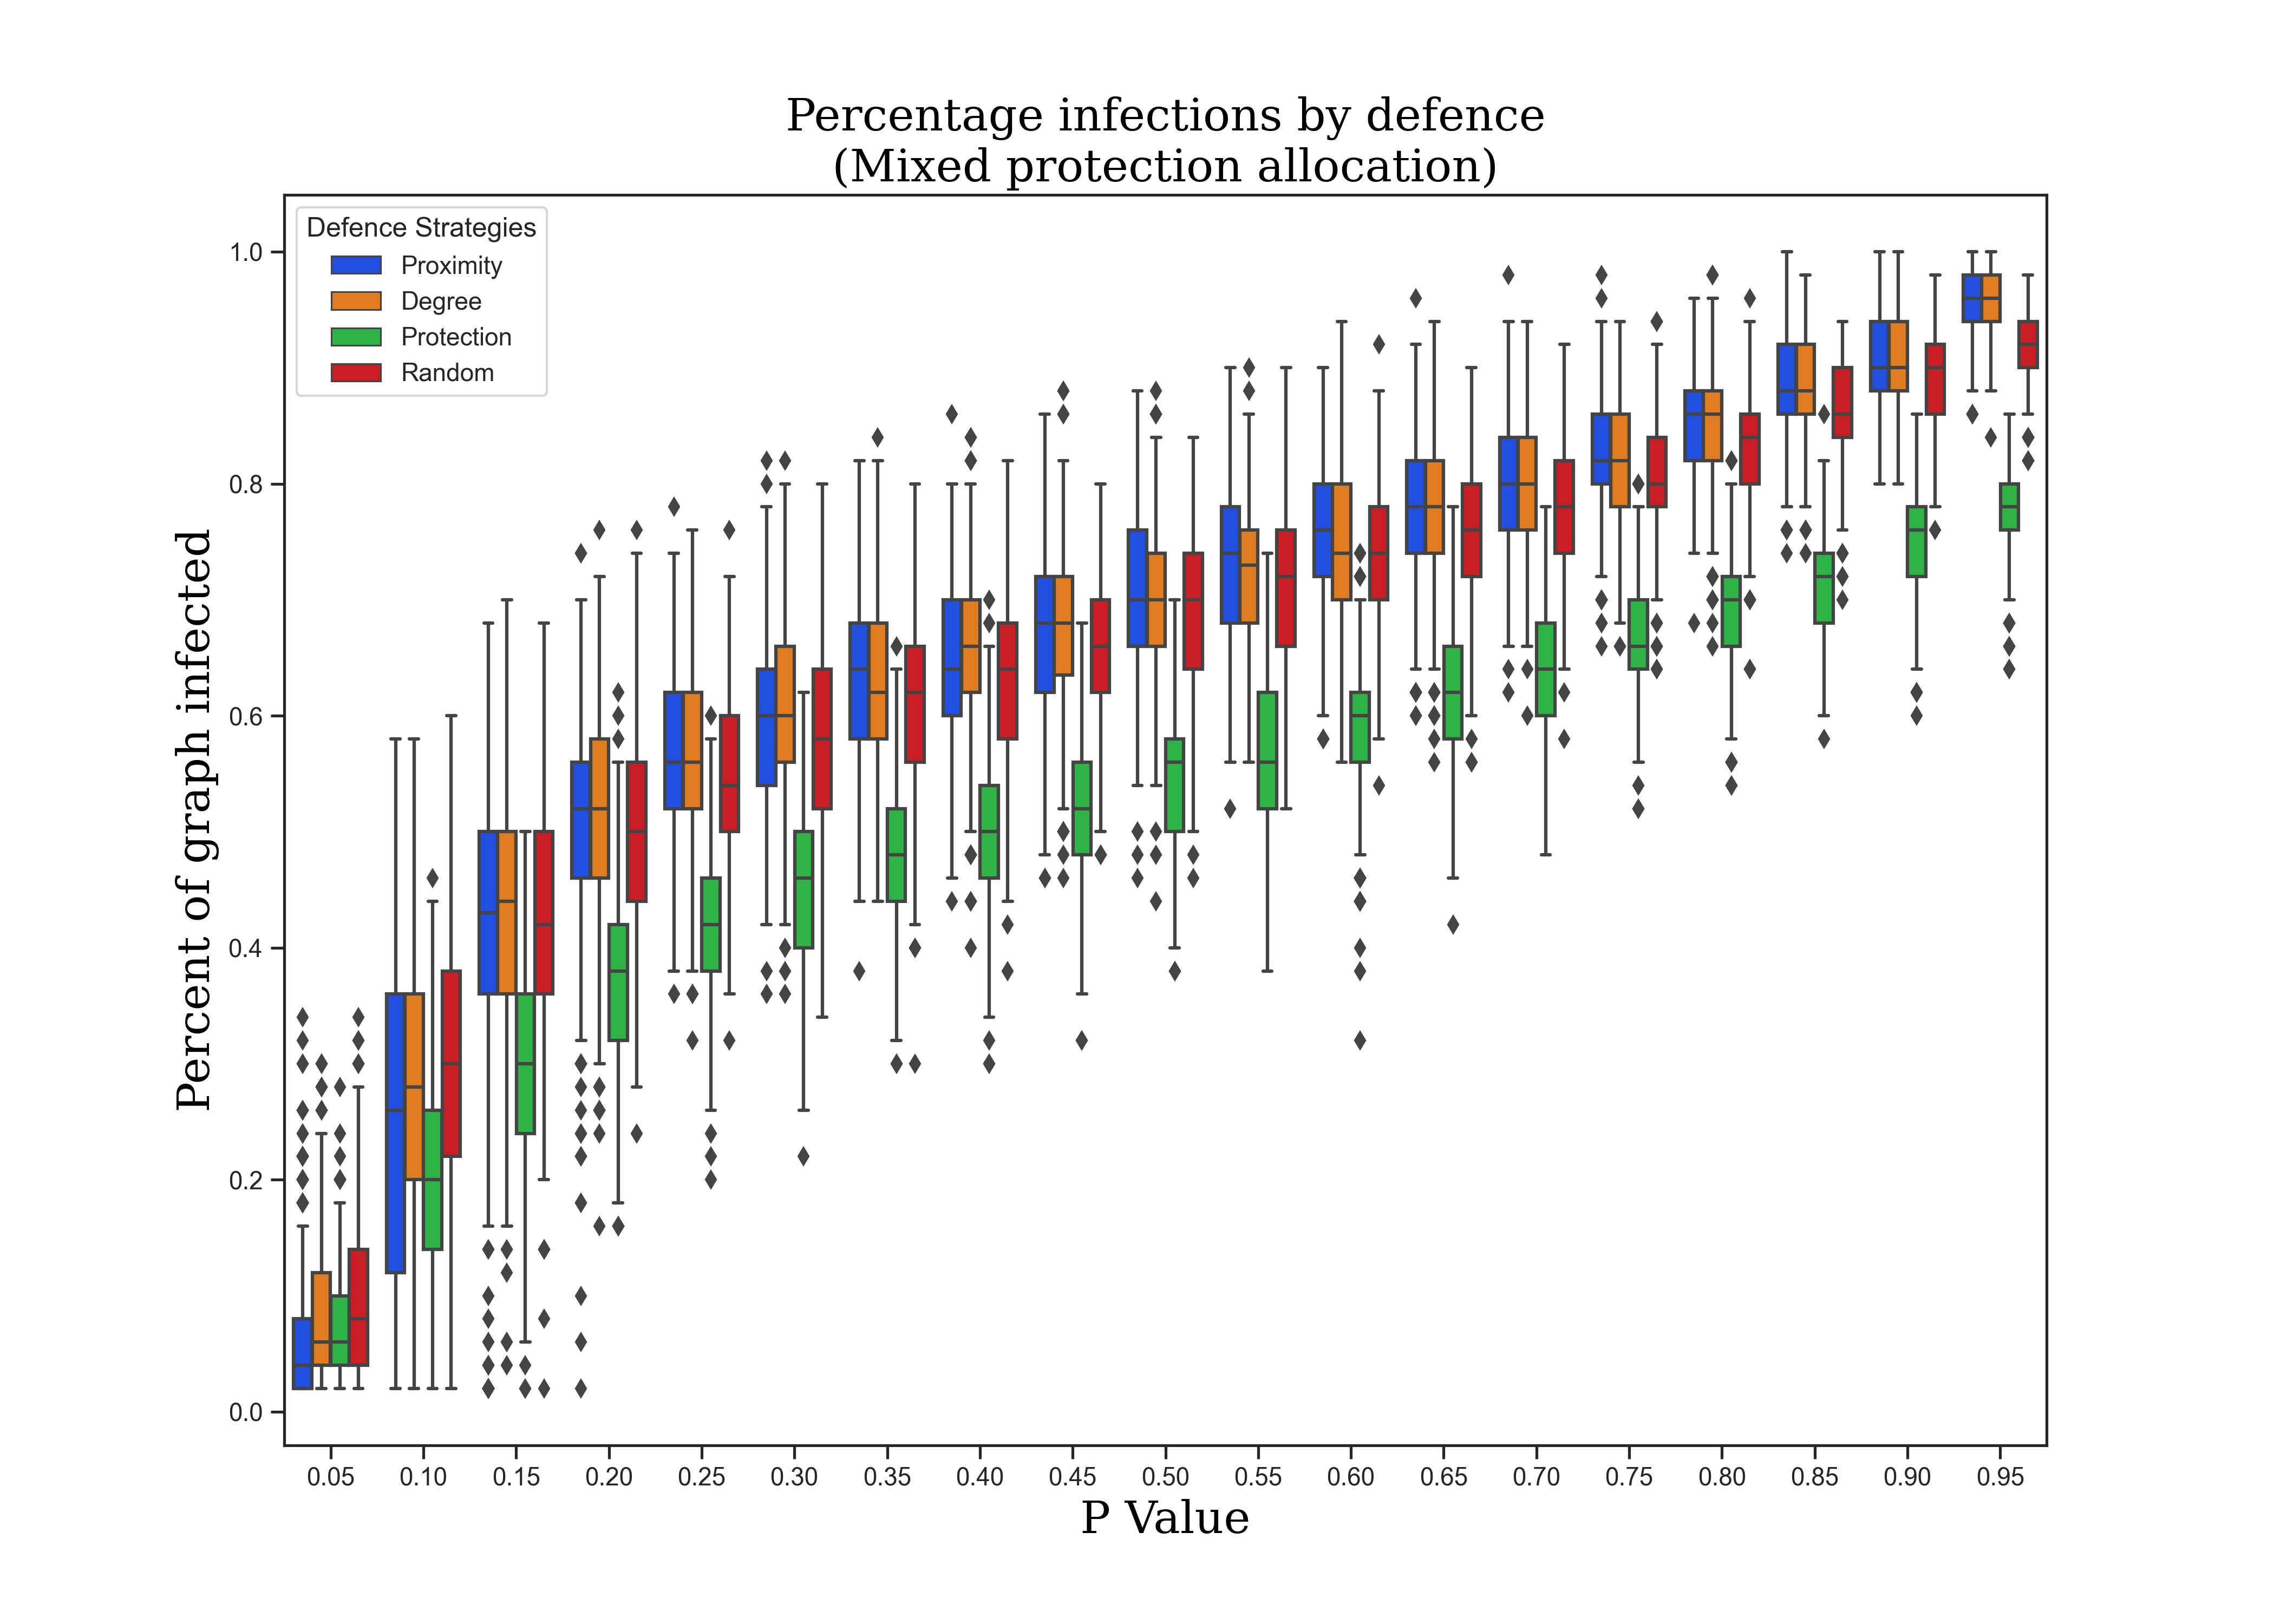
\includegraphics[height=0.8\textheight]{assets/charts/percent_infected/Mixed.jpg}
\end{frame}

% -----------------

%\begin{frame}{Mixed Protection}
%\centering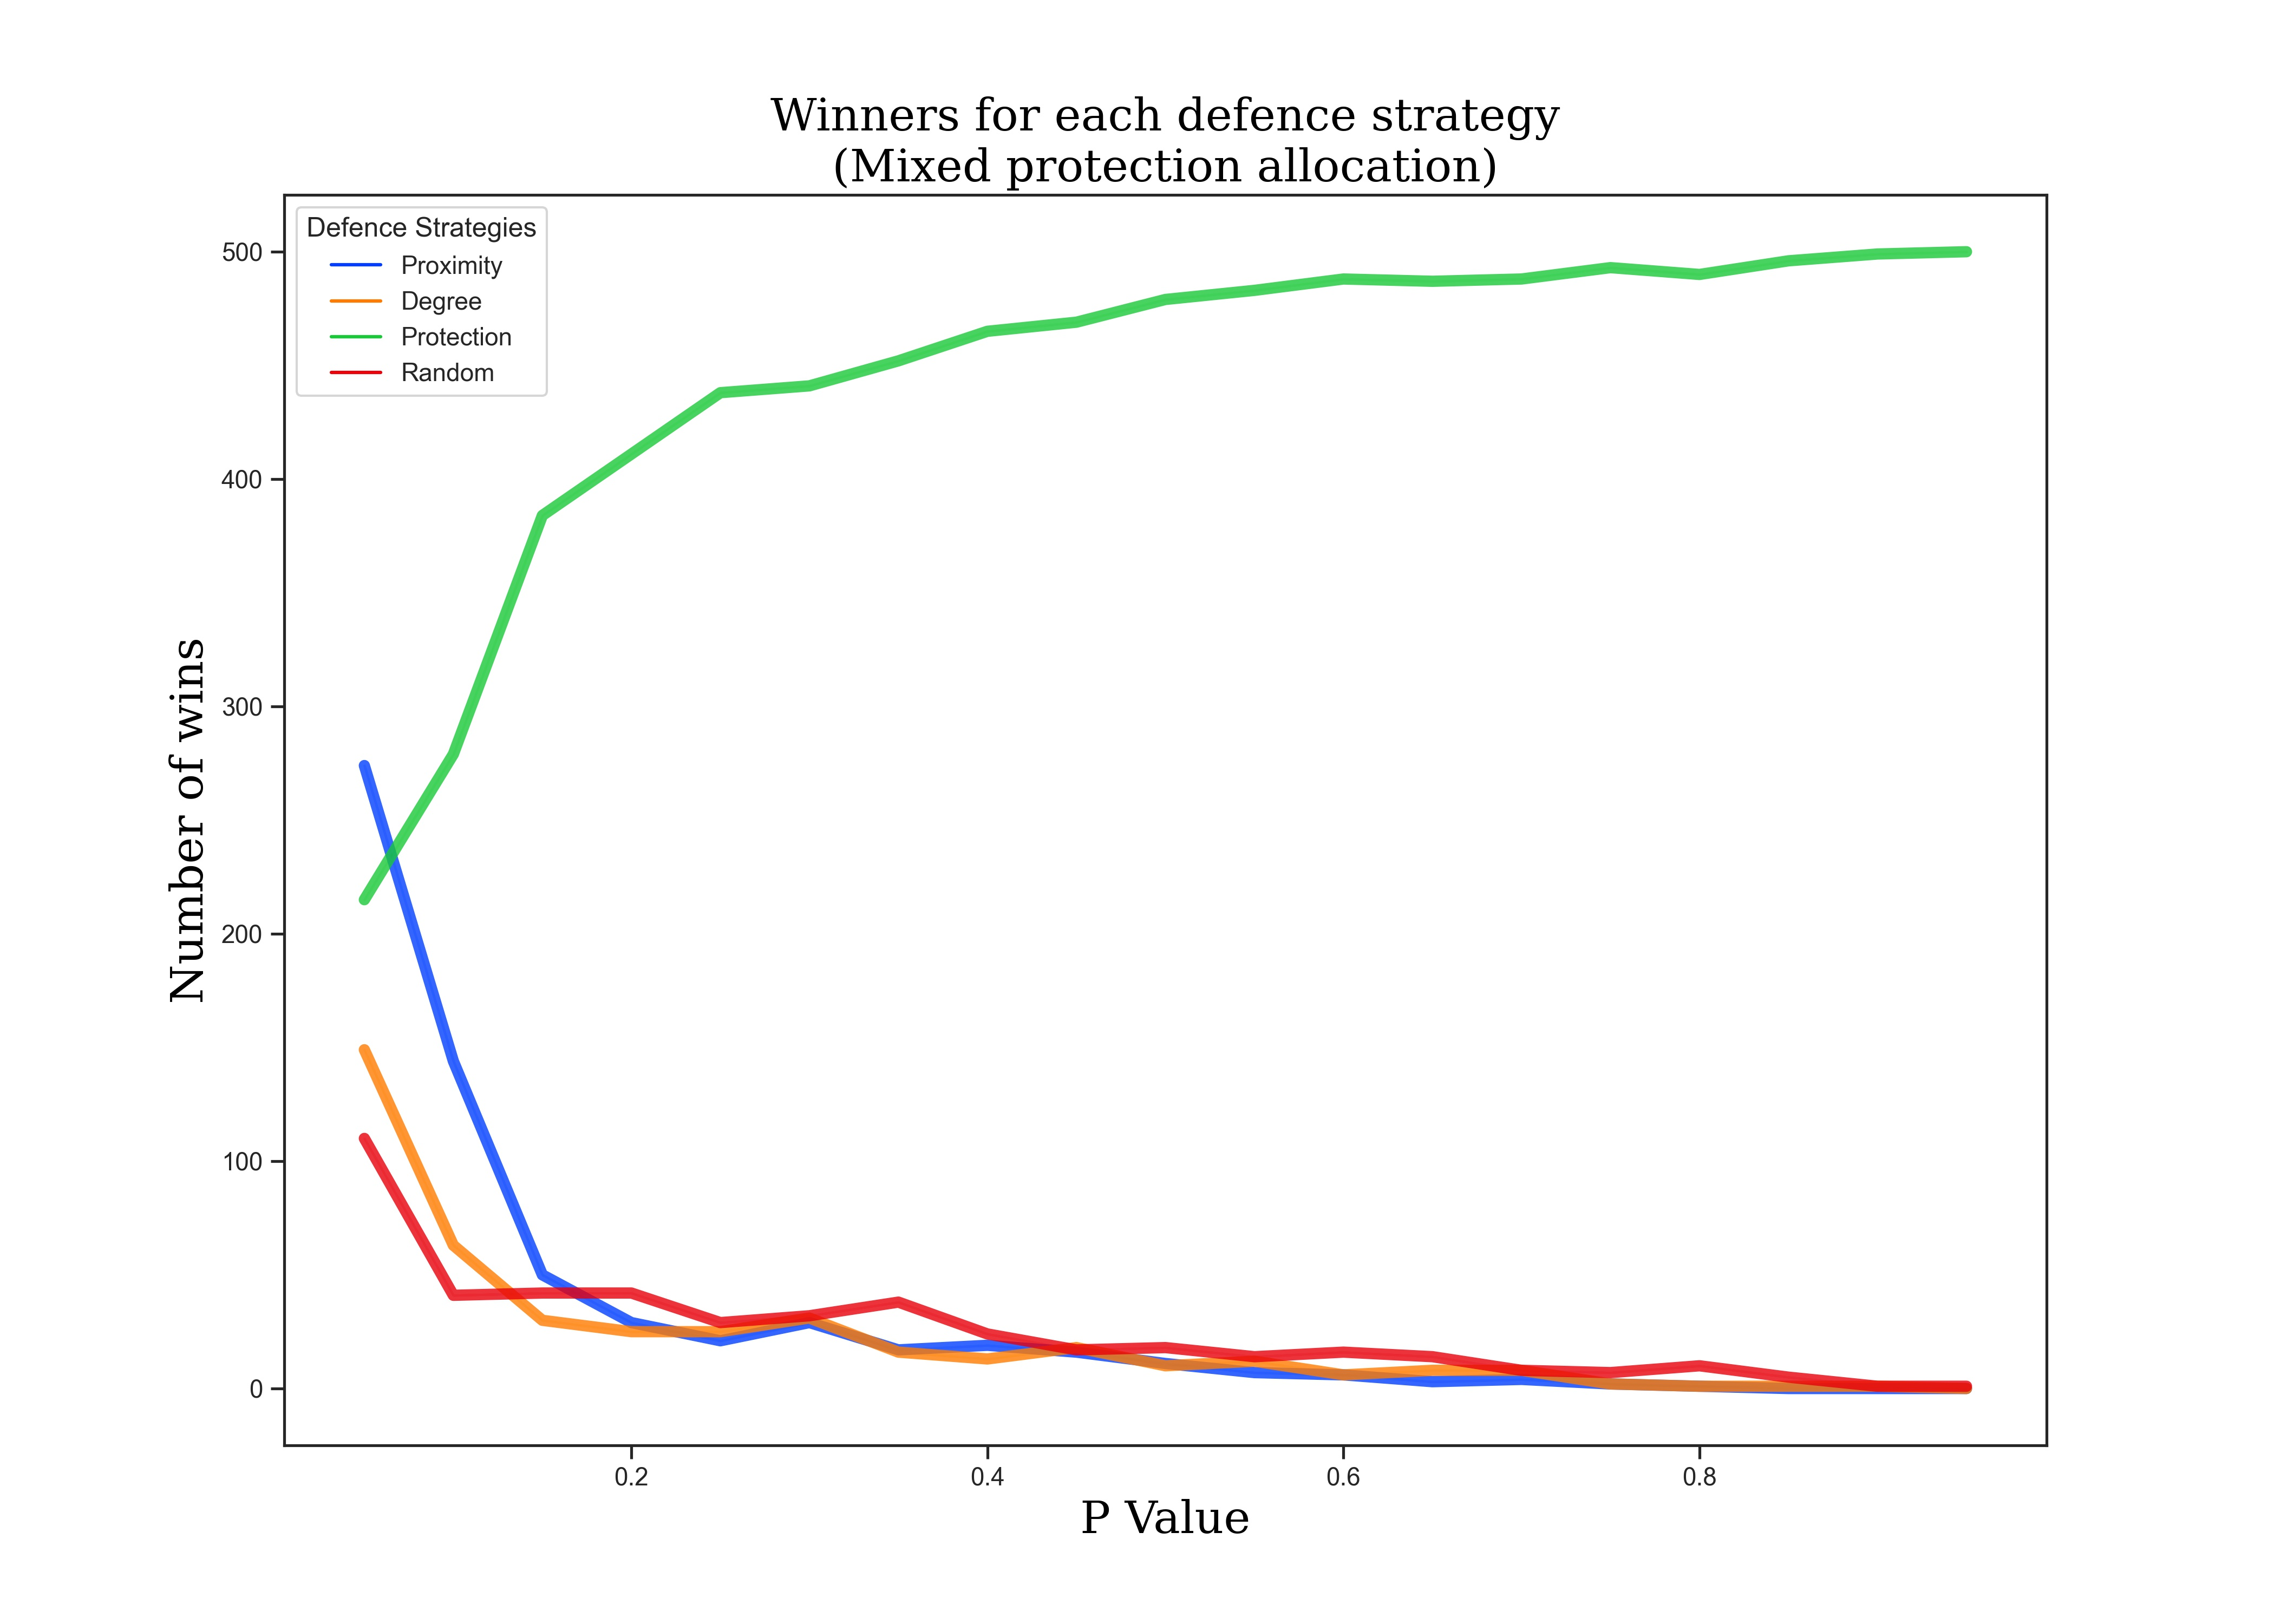
\includegraphics[height=0.8\textheight]{assets/charts/winners/Mixed.jpg}
%\end{frame}

% -----------------

\begin{frame}{Random Protection}
\centering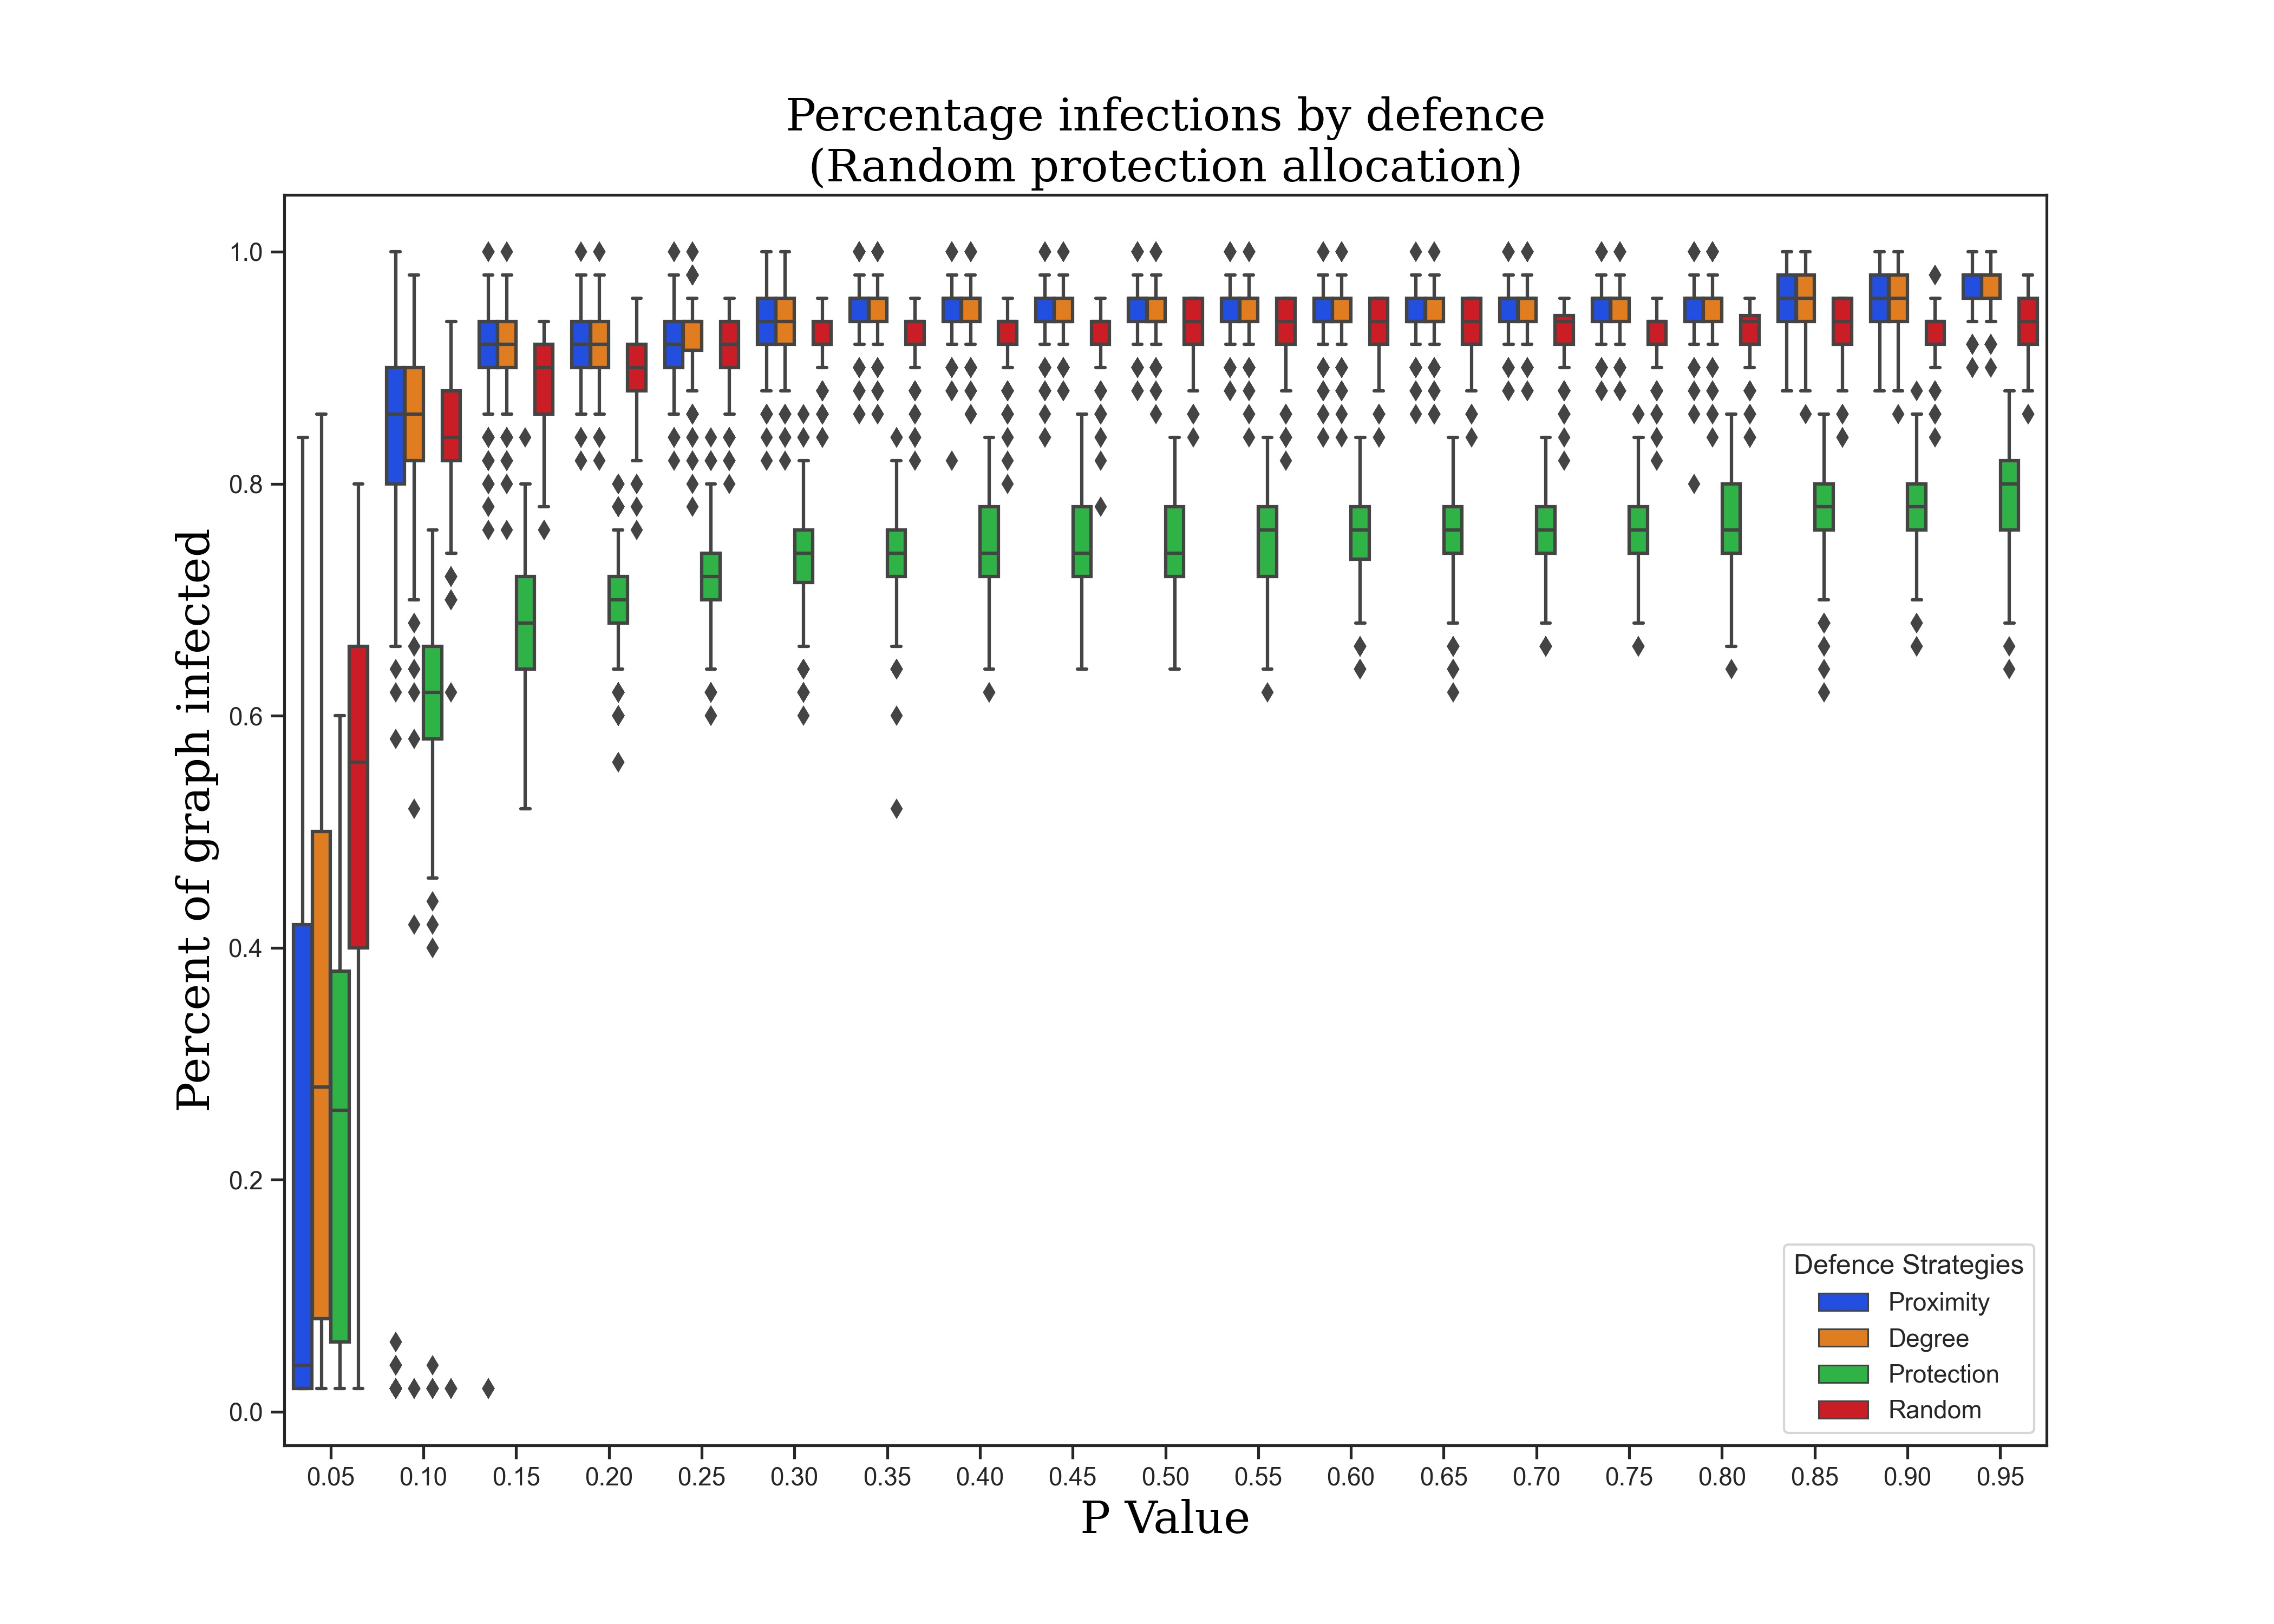
\includegraphics[height=0.8\textheight]{assets/charts/percent_infected/Random.jpg}
\end{frame}

% -----------------
%
%\begin{frame}{Random Protection}
%\centering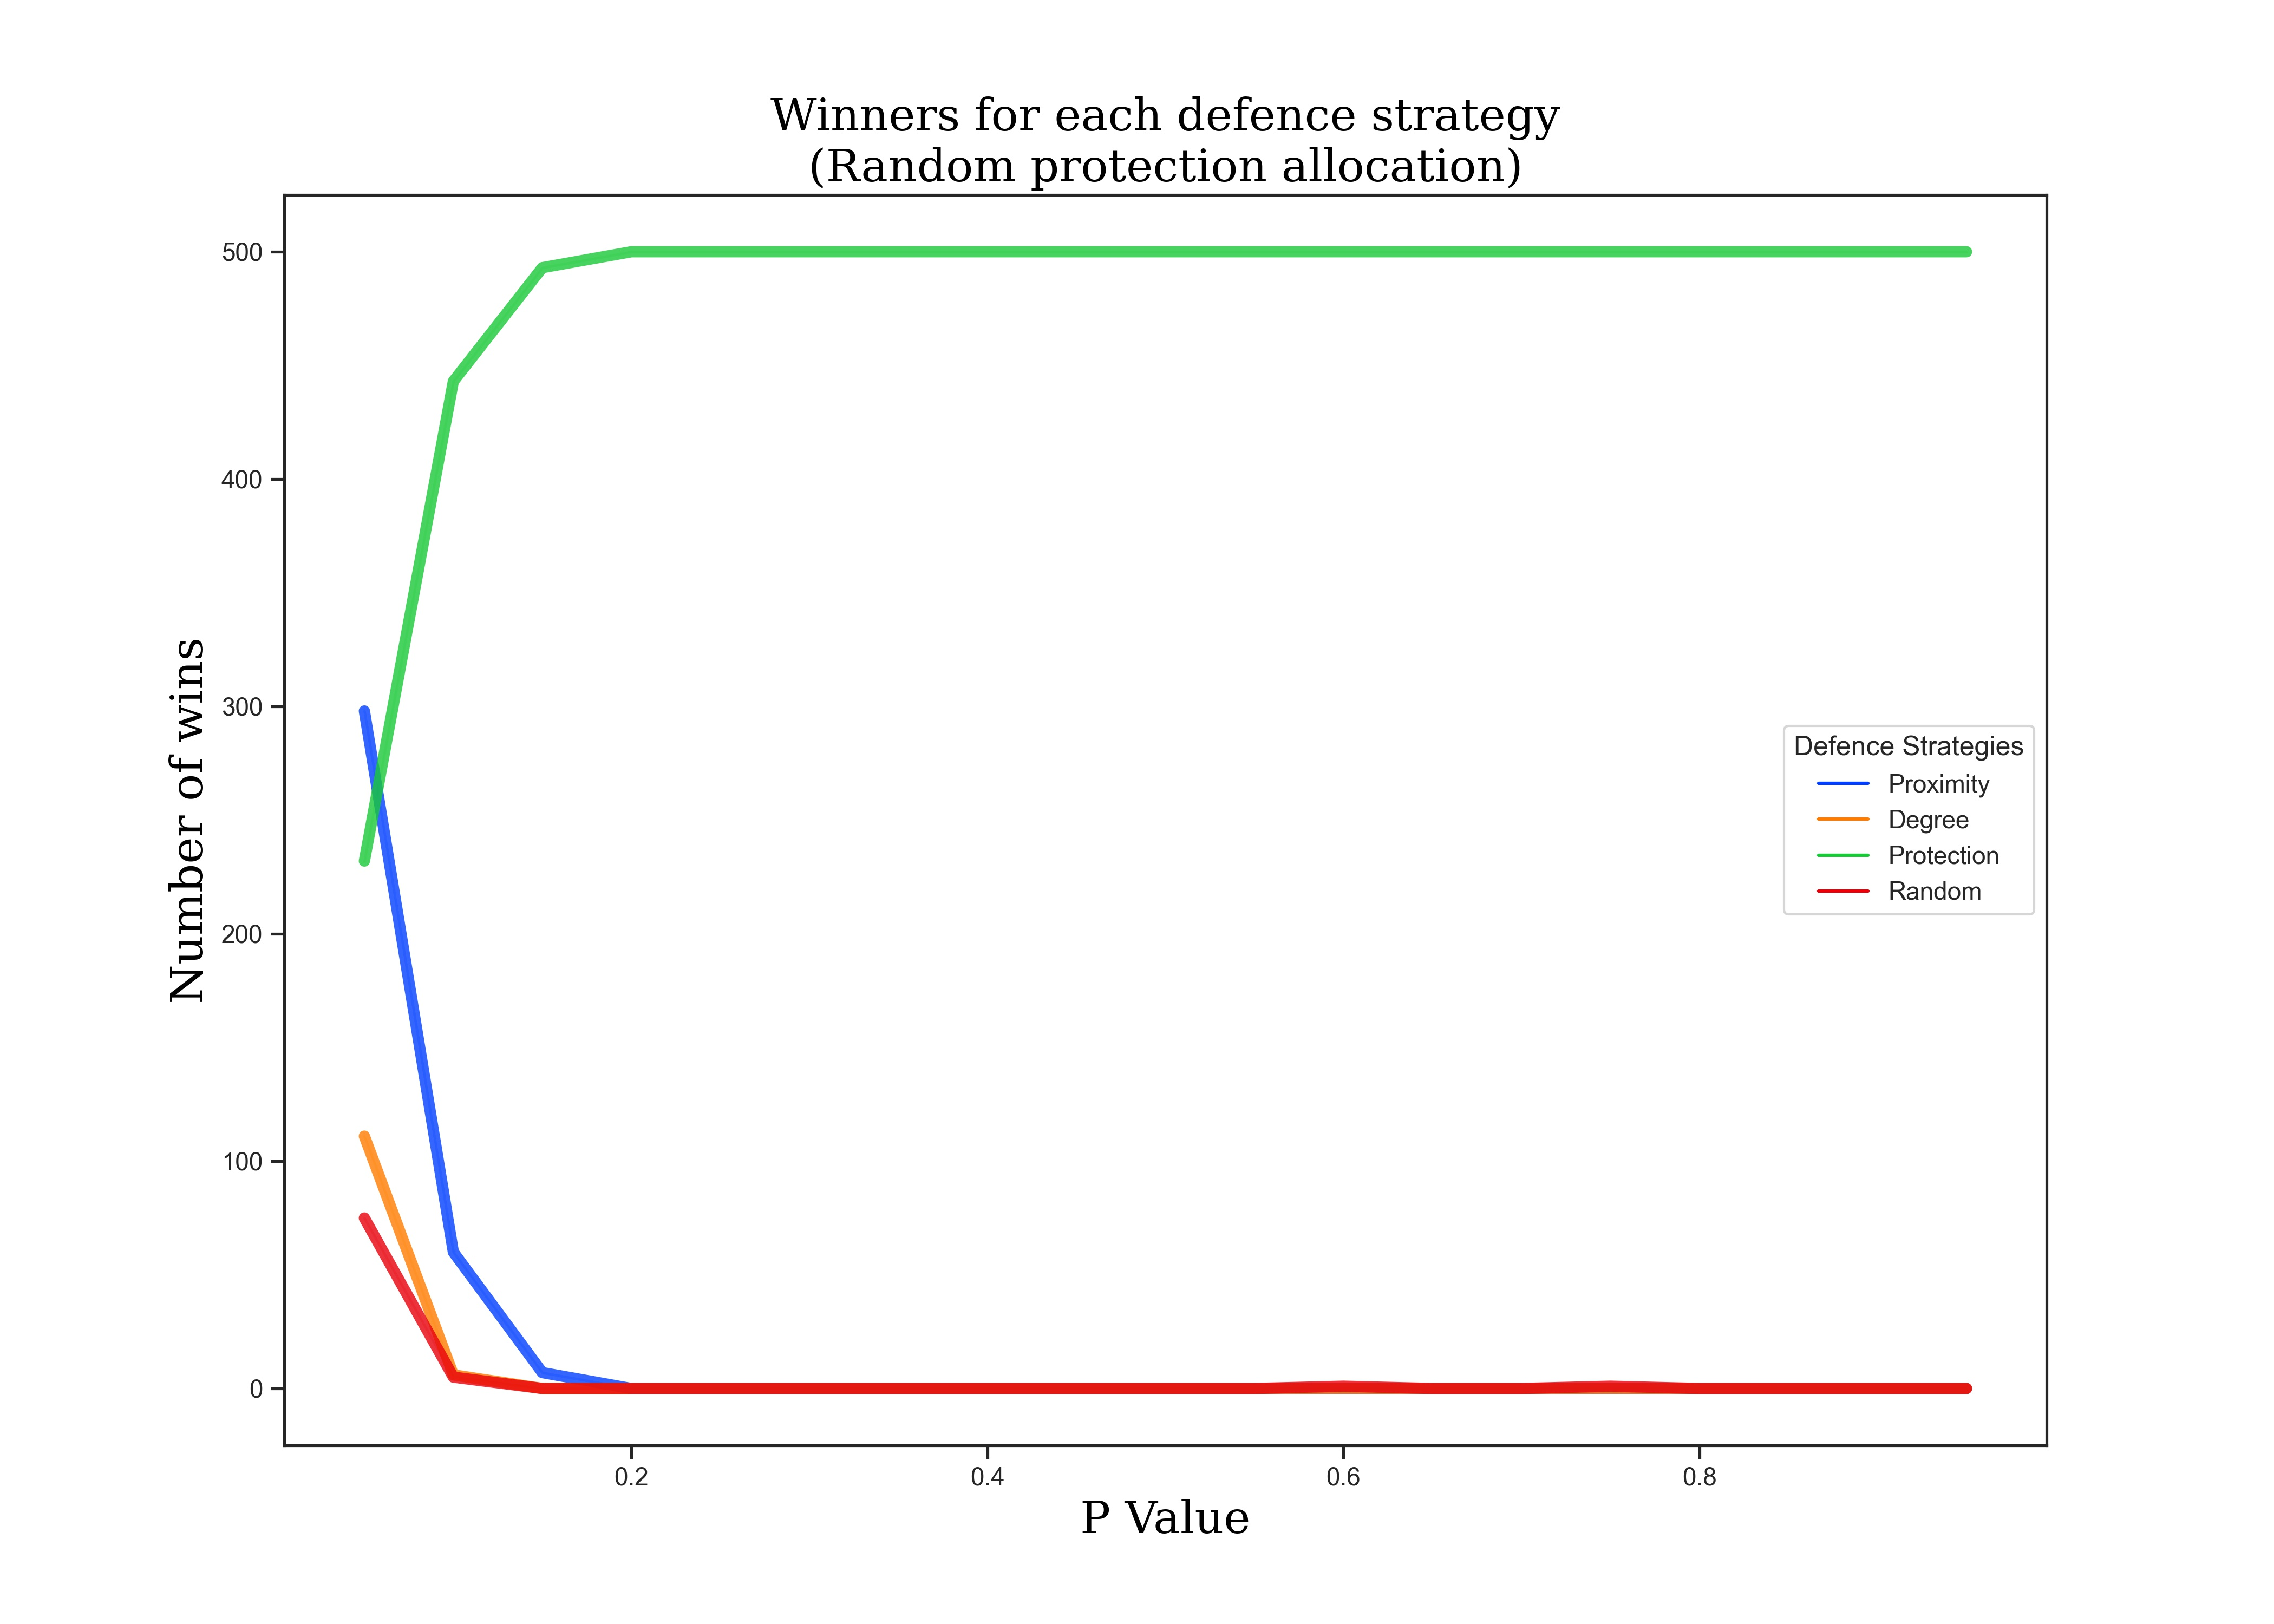
\includegraphics[height=0.8\textheight]{assets/charts/winners/Random.jpg}
%\end{frame}

% =============================================================================
%\section{Using Compartmental Frameworks}
%
%% -----------------------------------------------------------------------------
%\begin{frame}
%  \frametitle{Outline}
%  \tableofcontents[currentsection]
%\end{frame}
%
%% -----------------------------------------------------------------------------
%%\subsection{Standard $SIR$ model with fixed population}
%%
%%\begin{frame}
%%
%%The $SIR$ Model is a compartmental epidemiological model with three compartments (`states') related to an epidemic: {\it susceptible, infected} and {\it recovered.}
%%\begin{itemize}
%%	\pause
%%	\item $S(t)$ - people who don't have (but are able to contract) the infection at time $t$,
%%	\pause
%%	\item $I(t)$ - individuals who currently have the disease and are infectious,
%%	\pause
%%	\item $R(t)$ - people who have had the disease and have since recovered
%%	\pause
%%	\item For fixed population $N$, we have $S(t) + I(t) + R(t) = N$ - i.e. fixed population.
%%\end{itemize}
%%
%%\end{frame}
%%
%%% -----------------
%%
%%\begin{frame}
%%
%%Then, for rates of infection and recovery $\beta$ and $\gamma$ respectively, the standard $SIR$ model without vital dynamics is:
%%
%%\begin{align}
%%	\frac{dS}{dt} & = -\beta \frac{SI}{N} \label{dS}\\
%%	\frac{dI}{dt} & = \beta\frac{SI}{N} \gamma I \label{dI}\\
%%	\frac{dR}{dt} & = \gamma I - \mu R \label{dR}
%%\end{align}
%%
%%\end{frame}
%
%
%% -----------------------------------------------------------------------------
%\subsection{$SIR$ graph model} 
%\begin{frame}
%
%Examine probability of an agent being in a given state: 
%\begin{itemize}
%	\pause
%	\item $\langle A_i \rangle$ - time-independent probability of $i$ being in state $A$
%	\pause
%	\item $\langle A_i B_i \rangle$ - probability of $i$ and $j$ being in states $A$ and $B$ respectively.
%	\pause
%	\item $\beta_i$ - per-link infection rate for individual $i$.
%	\pause
%	\item $\gamma_i$ - recovery rate for $i$. 
%	\pause
%	\item For transmission matrix $T$, assign $T_{ij}=\beta_i$ if there is a route of infection between $i$ and $j$ ($T_{ij}=0$ otherwise). 
%	\pause
%	\item Often, we will consider unweighted and undirected graphs, but in general $T_{ij}$ may not equal $T_{ji}$.
%\end{itemize}
%
%\end{frame}
%
%% -----------------
%
%\begin{frame}
%
%We can replace $\beta_i$ with a term involving a transmission matrix of a network to begin extending the usual $SIR$ model into a network realm. 
%%Using the substitution $ \beta_i \frac{SI}{N} = \sum^{N}_{j=1}T_{ij} \langle S_i I_j \rangle,$ the equations become
%\begin{align*}
%\dot{\langle S_i \rangle} & = -\sum^{N}_{j=1}T_{ij} \langle S_i I_j \rangle\\
%\dot{\langle I_i \rangle} & =\sum^{N}_{j=1}T_{ij}\langle S_i I_j \rangle - \gamma_i \langle I \rangle \\
%\dot{\langle R_i \rangle} & = \gamma_i \langle I \rangle,
%\end{align*}
%which are the evolution equations given in \cite{kiss_2014}.
%
%\end{frame}
%
%% ----------------------------------------------------------------------------
%
%\subsection{Adding a new state}
%
%\begin{frame}{Protected State}
%\begin{itemize}
%	\item $\zeta_i$ - probability that we defend individual $i$,
%	\item $\alpha_i$ - efficacy of the protection measure for individual $i$ (may decay over time and vary from person to person). 	
%\end{itemize}
%\pause
%Using these rates of protection and effectiveness, for fixed population size the differential equations become:
%\pause
%\begin{align}
%\dot{\langle S_i \rangle} & = \alpha_i \langle P_i \rangle - \sum^{N}_{j=1}T_{ij} \langle S_i I_j \rangle - \zeta_i\langle S_i \rangle\\
%\dot{\langle I \rangle} & =\sum^{N}_{j=1}T_{ij}\langle S_i I_j \rangle - \gamma_i \langle I \rangle \\
%\dot{\langle R_i \rangle} & = \gamma_i \langle I \rangle \\
%\dot{\langle P_i \rangle} & = \zeta_i \langle S_i \rangle - \alpha_i \langle P_i \rangle.
%\end{align} 
%
%\end{frame}

% -----------------

% =============================================================================

%\section{Describing Compartmental Graph Models Exactly}
%
%% -----------------------------------------------------------------------------
%\begin{frame}
%  \frametitle{Outline}
%  \tableofcontents[currentsection]
%\end{frame}
%
%% -----------------------------------------------------------------------------
%\subsection{Required Equations}
%
%\begin{frame}{Numbers of Equations}
%
%\begin{columns}
%\begin{column}{0.5\textwidth}
%Consider the triangle graph. The equations required to precisely express the system $SIR$ dynamics of this network are as below \cite{kiss_2014}.
%\end{column}
%
%\begin{column}{0.5\textwidth}
%\centering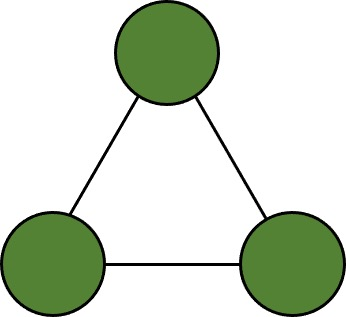
\includegraphics[width=0.4\textwidth]{assets/triangle}
%\end{column}
%\end{columns}
%
%\begin{align}
%\text{6 singles: } & \dot{\langle S_1 \rangle}, \dot{\langle S_2 \rangle}, \dot{\langle S_3 \rangle}, \dot{\langle I_1 \rangle}, \dot{\langle I_2 \rangle}, \dot{\langle I_3 \rangle}.\label{eq:SIRsingle}\\
%\text{6 doubles: } & \dot{\langle S_1 I_2 \rangle},\dot{\langle I_1 S_2 \rangle}, \dot{\langle S_1 I_3 \rangle}, \dot{\langle I_1 S_3 \rangle}, \dot{\langle S_2 I_3\rangle}, \dot{\langle I_2 S_3 \rangle}.\label{eq:SIRdouble}\\
%\text{6 triples: } & \dot{\langle S_1 I_2 I_3 \rangle}, \dot{\langle S_1 I_2 S_3 \rangle}, \dot{\langle S_1 S_2 I_3 \rangle}, \dot{\langle I_1 S_2 S_3 \rangle}, \dot{\langle I_1 I_2 S_3 \rangle}, \dot{\langle I_1 S_2 I_3 \rangle}. \label{eq:SIRtriple}
%\end{align}
%
%\end{frame}
%
%% -----------------
%
%\begin{frame}
%
%Using the equations for the $SIRP$ model, we have the following equation requirements:
%\begin{align*}
%\text{9 singles: (} \ref{eq:SIRsingle} \text{) and } & \dot{\langle P_1 \rangle}, \dot{\langle P_2 \rangle}, \dot{\langle P_3 \rangle}.\\
%\text{18 doubles: (} \ref{eq:SIRdouble} \text{) and }& \dot{\langle S_1 P_2 \rangle},\dot{\langle P_1 S_2 \rangle}, \dot{\langle I_1 P_2 \rangle}, \dot{\langle P_1 I_2 \rangle}, \dot{\langle S_1 P_3\rangle}, \dot{\langle P_1 S_3 \rangle},\\ & \dot{\langle I_1 P_3 \rangle}, \dot{\langle P_1 I_3 \rangle}, \dot{\langle S_2 P_3 \rangle}, \dot{\langle P_2 S_3 \rangle}, \dot{\langle I_2 P_3 \rangle}, \dot{\langle P_2 I_3 \rangle}. \\
%\text{24 triples: (} \ref{eq:SIRtriple} \text{) and } & \dot{\langle S_1 S_2 P_3 \rangle}, \dot{\langle S_1 P_2 S_3 \rangle}, \dot{\langle S_1 I_2 P_3\rangle}, \dot{\langle S_1 P_2 I_3 \rangle}, \dot{\langle S_1 P_2 P_3\rangle}, \\
%& \dot{\langle I_1 S_2 P_3 \rangle}, \dot{\langle I_1 P_2 S_3 \rangle}, \dot{\langle I_1 I_2 P_3 \rangle}, \dot{\langle I_1 P_2 I_3 \rangle}, \dot{\langle I_1 P_2 P_2 \rangle},\\
%& \dot{\langle P_1 S_2 S_3 \rangle}, \dot{\langle P_1 S_2 I_3 \rangle}, \dot{\langle P_1 I_2 S_3 \rangle}, \dot{\langle P_1 I_2 I_3 \rangle}, \dot{\langle P_1 P_2 I_3 \rangle}, \\
%& \dot{\langle P_1 P_2 S_3 \rangle}, \dot{\langle P_1 S_2 P_3 \rangle},  \dot{\langle P_1 I_2 P_3\rangle}.
%\end{align*}
%
%\end{frame}

% -----------------------------------------------------------------------------
%\subsection{Closures}
%
%\begin{frame}{What are closures?}
%
%\begin{itemize}
%	\pause
%	\item In the previous section, we saw equations for singles 
%	\pause
%	\item We have also seen equations needed for the triangle network (including doubles and triples)
%	\pause 
%	\item How many equations do we need in general?
%\end{itemize}
%\pause
%The number of other equations will usually increase when we require closures, as closure equations will sometimes require equations that we don't usually consider as they are dynamically uninteresting, e.g. $\langle S_i S_j \rangle$ where $i$ and $j$ are adjacent.
%
%\end{frame}
%
%% -----------------
%
%\begin{frame}
%
%Consider the equations below for calculating singles and pairs:
%\begin{align*}
%\langle \dot{S_i} \rangle & = -\sum^N_{j=1}T_{ij}\langle S_iI_j\rangle,\\
%\langle\dot{I_i}\rangle & = \sum^N_{j=1}T_{ij}\langle S_iI_j\rangle - \gamma_i\langle I_i \rangle,\\
%\langle\dot{S_iI_j}\rangle & = \sum^N_{k=1,k\neq i}T_{jk}\langle S_i S_j I_k \rangle - \sum^N_{k=1,k\neq j}T_ik\langle I_k S_i I_j \rangle \\ 
%			    	      & ~~~~~~~~~~~~~~~~~- T_{ij}\langle S_iI_j \rangle - \gamma_i\langle S_i I_j \rangle,\\
%\langle \dot{S_i S_j}\rangle & = - \sum^N_{k=1,k\neq j}T_{ik}\langle I_k S_i S_j \rangle - \sum^N_{k=1,k\neq i}T_{jk}\langle S_i S_j I_k \rangle,
%\end{align*}
%
%\end{frame}
%
%% -----------------
%
%\begin{frame}
%
%\begin{align*}
%\langle \dot{S_i} \rangle & = -\sum^N_{j=1}T_{ij}\langle S_iI_j\rangle,\\
%\langle\dot{I_i}\rangle & = \sum^N_{j=1}T_{ij}\langle S_iI_j\rangle - \gamma_i\langle I_i \rangle,\\
%\langle\dot{S_iI_j}\rangle & = \sum^N_{k=1,k\neq i}T_{jk}\highlight{\langle S_i S_j I_k \rangle} - \sum^N_{k=1,k\neq j}T_ik\highlight{\langle I_k S_i I_j \rangle} \\ 
%			    	      & ~~~~~~~~~~~~~~~~~- T_{ij}\langle S_iI_j \rangle - \gamma_i\langle S_i I_j \rangle,\\
%\langle \dot{S_i S_j}\rangle & = - \sum^N_{k=1,k\neq j}T_{ik}\highlight{\langle I_k S_i S_j \rangle} - \sum^N_{k=1,k\neq i}T_{jk}\highlight{\langle S_i S_j I_k \rangle},
%\end{align*}
%
%This is {\it not} a closed system - we require equations for triples.
%
%\end{frame}
%
%% -----------------
%
%\begin{frame}
%\centering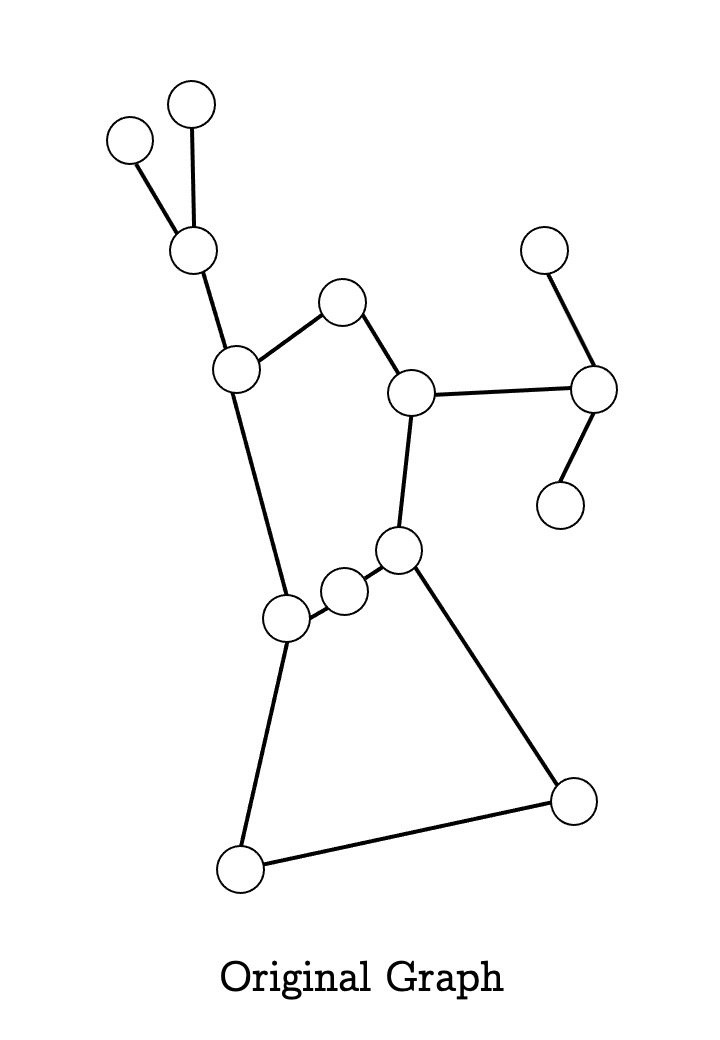
\includegraphics[height=0.9\textheight]{assets/eg-cutvertex/0}
%\end{frame}
%
%% -----------------
%
%\begin{frame}
%\centering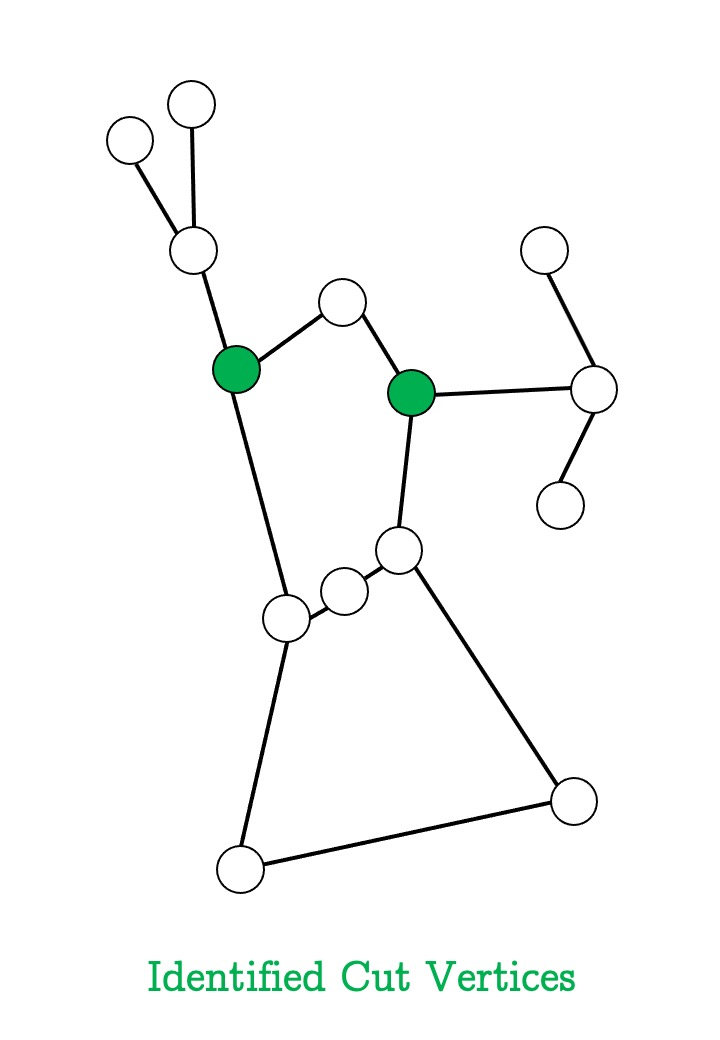
\includegraphics[height=0.9\textheight]{assets/eg-cutvertex/1}
%\end{frame}
%
%% -----------------
%
%\begin{frame}
%\centering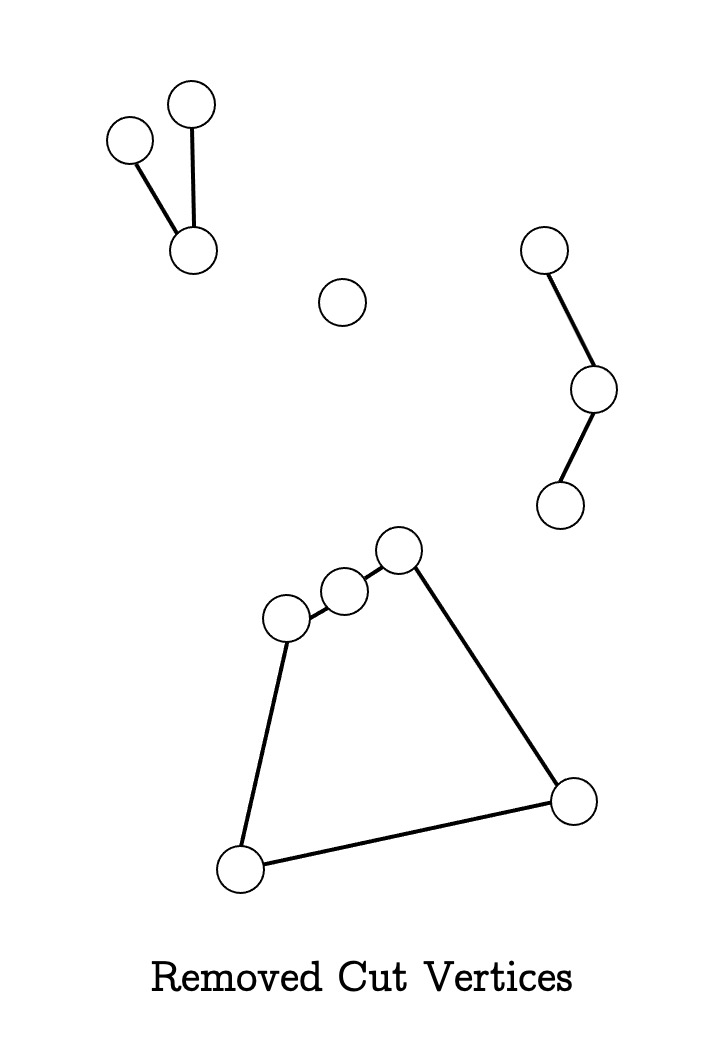
\includegraphics[height=0.9\textheight]{assets/eg-cutvertex/2}
%\end{frame}
%
%% -----------------
%
%\begin{frame}
%\centering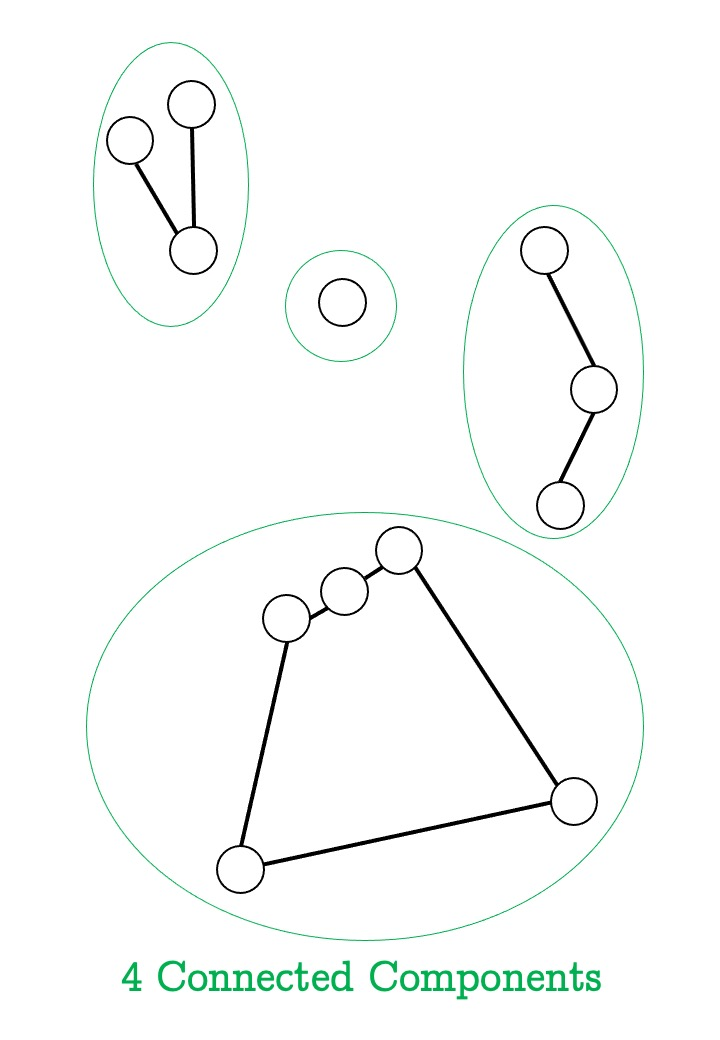
\includegraphics[height=0.9\textheight]{assets/eg-cutvertex/3}
%\end{frame}
%
%% -----------------
%
%\begin{frame}{Calculating Closures from Cut-Vertex Sets}
%
%Let $G = \{V,E\}$ be a graph on $N$ vertices. \pause Consider a connected subset of vertices $F = {v_1,v_2,\dots,v_k}\subset V$ \pause and assume $\exists v_{i^\ast} \in F$ a cut-vertex in $G$, such that $F \setminus \{v_{i^\ast}\}$ is partitioned into at least two disjointed components with vertices $F_1 = {v_1, v_2,\dots, v_{i-1}}$ and $F_2 = {v_{i+1}, v_{i+2},\dots, v_k}$ belonging to any such two, distinct and disjointed components or subnetworks. \pause Then the following equation holds:
%
%\begin{align*}
%\langle Z_{v_1} Z_{v_2},& \dots Z_{v_{i-1}} S_{v_i^\ast} Z_{v_{i+1}} \dots Z_{v_k} \rangle (t) = \\
%&\frac{\langle Z_{v_1} Z_{v_2} \dots Z_{v_{i-1}} S_{v_i^\ast}\rangle(t)\langle S_{v_i^\ast} Z_{v_{i+1}} \dots Z_{v_k} \rangle}{\langle S_{v_i^\ast} \rangle (t)}
%\end{align*}
%
%where $Z_{v_i} \in \{S, I\}~\forall v_i \neq v_{i^\ast}$. \cite{kiss_2014}
%
%\end{frame}
%
%% -----------------
%
%\begin{frame}{Bounding}
%Denote by $\text{Ind}(v_{i_j})$ for $j=1,2,\dots,L$ the number of subgraph $v_{i_j}$ belongs to.\\
%\textbf{Upper bound:}
%\begin{equation*}
%N_{EQ}(G) = \sum^P_{i=1}m_if_i-2\sum^L_{j=1}(\text{Ind}(v_{i_j})-1).
%\end{equation*}
%We take a sum across number of equations for all subgraphs and subtract unnecessary multiplications from cut-vertices being replaced into produced sub-graphs. \cite{kiss_2014}
%
%\end{frame}
%
%% -----------------
%
%\begin{frame}{Bounding}
%\textbf{Upper bound:}
%\begin{equation*}
%N_{EQ}(G) = \sum^P_{i=1}\highlight{m_i}f_i-2\sum^L_{j=1}(\text{Ind}(v_{i_j})-1).
%\end{equation*}
%Note: $m_i$ denotes the number of equations required for subnetwork $i$, e.g.
%\begin{itemize}
%	\item An edge requires 7 equations (4 for singles, 3 for pairs)
%	\item A triangle requires 22 equations
%	\item A cycle on 4 vertices requires 45 equations
%\end{itemize}
%\end{frame}
%
%% -----------------
%
%\begin{frame}
%We can in fact bound these multipliers. From the requirements of a subgraph (connected, no cut vertices), for a number of vertices $n$ our worst-case scenario is the complete graph (everything is connected to everything else) and our best-case scenario is the cycle on $n$ vertices.
%
%%\pause
%%\begin{figure}
%%\centering
%%  \begin{subfigure}{0.5\textwidth}
%%    \centering
%%    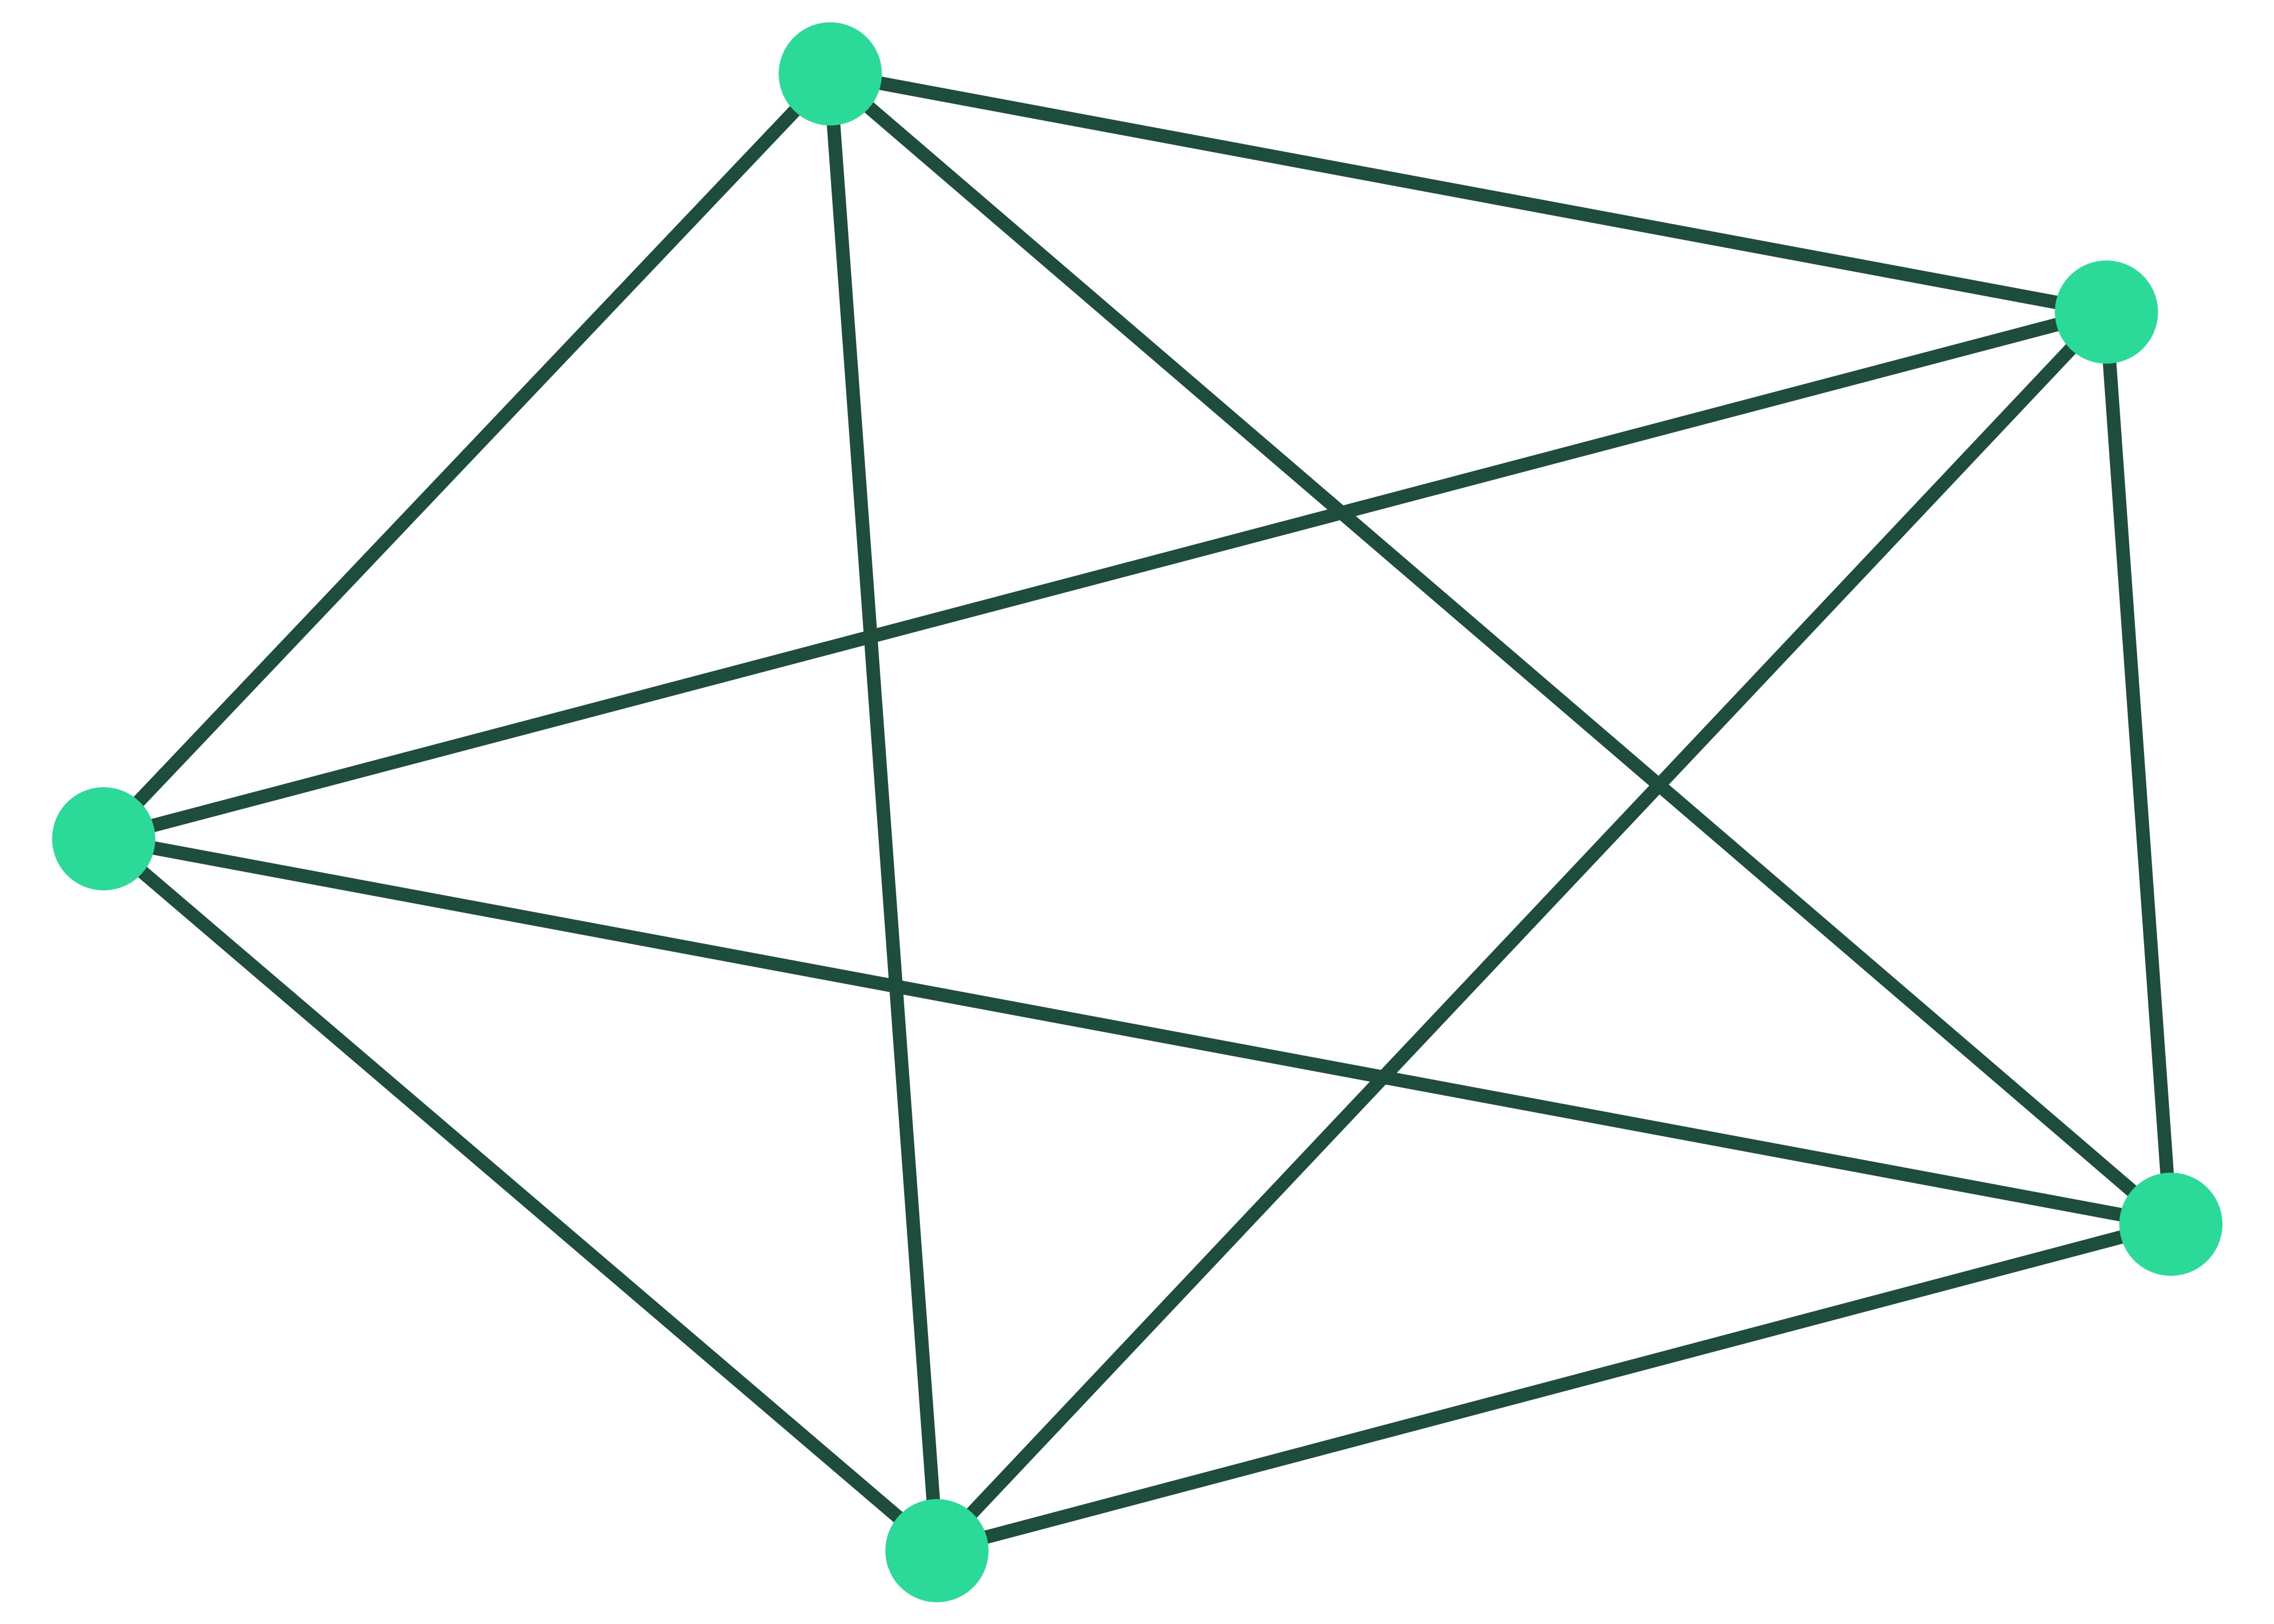
\includegraphics[width=0.45\textwidth]{assets/complete}
%%    \caption{Number of equations: X}
%%  \end{subfigure}%
%%\pause
%%  \begin{subfigure}{.5\textwidth}
%%  \centering
%%    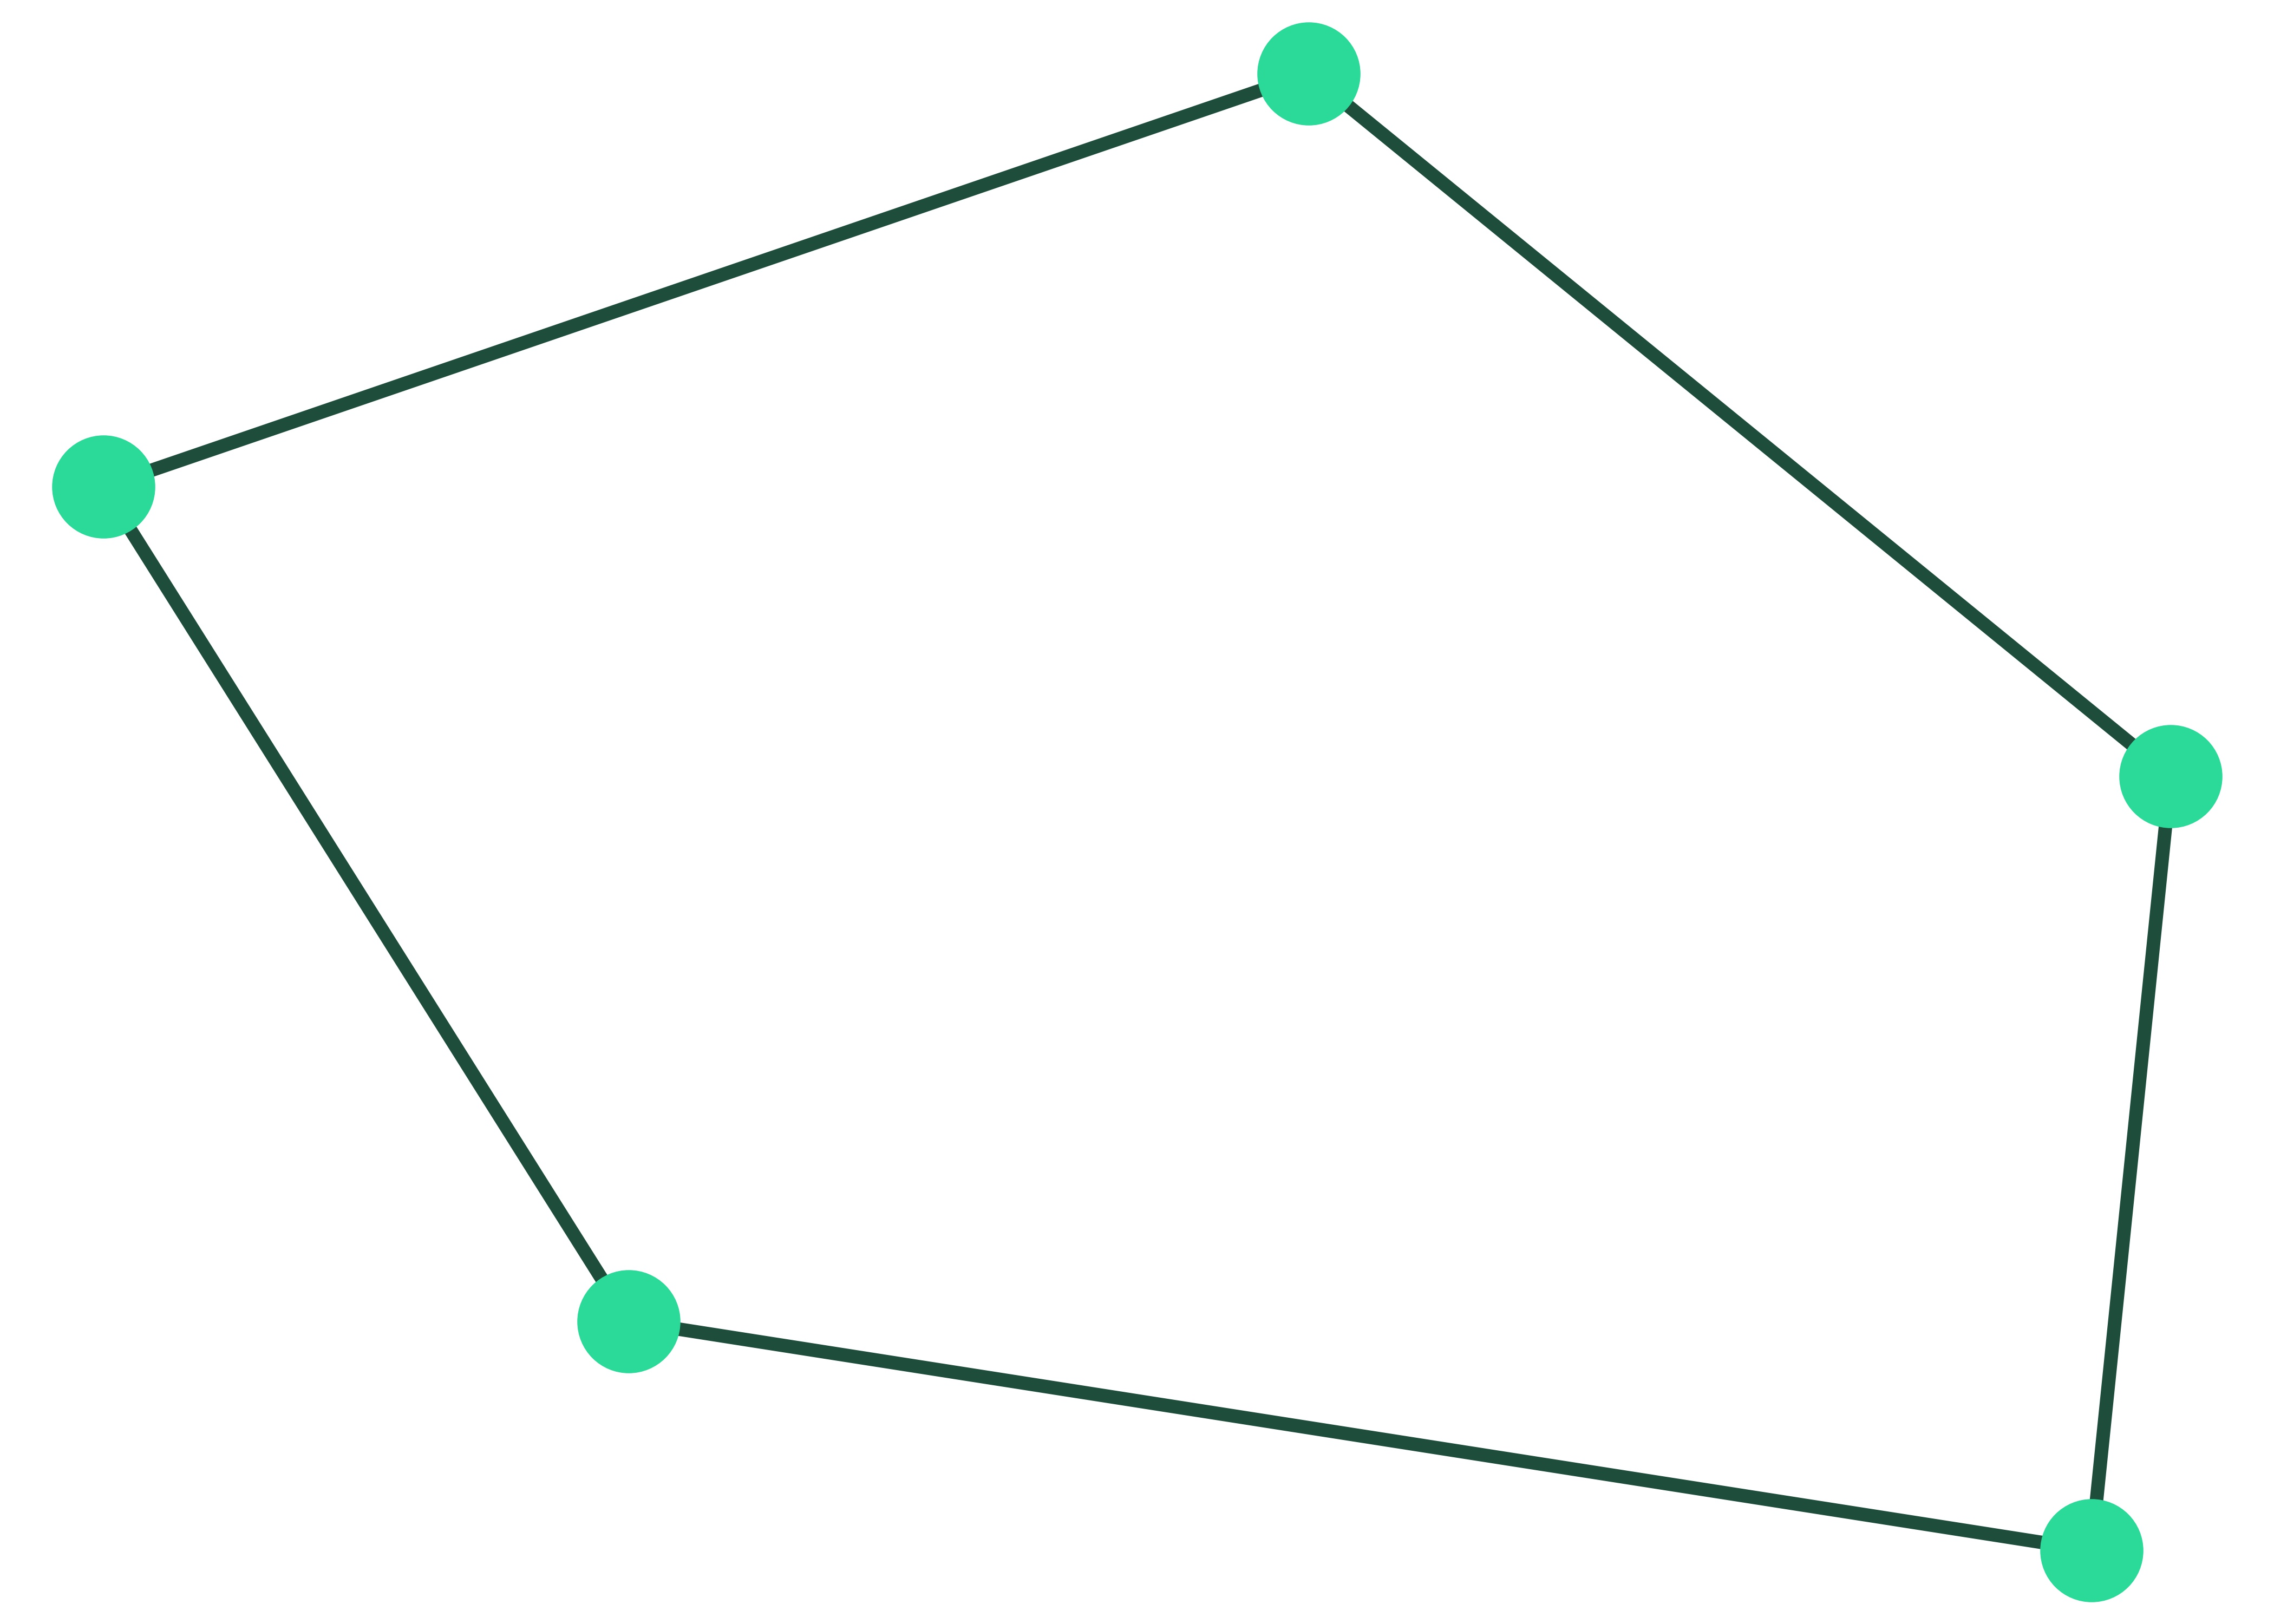
\includegraphics[width=0.49\textwidth]{assets/cycle}
%%    \caption{Number of Equations: Y}
%%  \end{subfigure}
%% \caption{Best and Worst Case Scenarios}
%%\end{figure}
%
%\end{frame}

% =============================================================================
\section{Conclusion}

% -----------------------------------------------------------------------------
\begin{frame}
\frametitle{Outline}
\tableofcontents[currentsection]
\end{frame}


% -----------------------------------------------------------------------------
\begin{frame}

We discussed:

\begin{itemize}
	\item Some fundamentals of Graph Theory, including {\scshape Firefighter}
	\item Using {\scshape Firefighter} as a model for disease spread
	\item Failings of this approach to disease modelling
	\item How agency can address these issues
\end{itemize}

\end{frame}

\begin{frame}{References}
\bibliographystyle{siam}
\nocite{*}
\bibliography{slides-bib}
\end{frame}


% =============================================================================
% Back slide.
{
  \usebackgroundtemplate{
\includegraphics[height=\paperheight]{assets/title-slide}}

  \begin{frame}[plain]

    \begin{columns}

      \begin{column}[l]{5cm}
      \end{column}

      \begin{column}[r]{5cm}
        \textcolor{white}{
          Questions?
        }
      \end{column}

    \end{columns}
  \end{frame}
}


\end{document}
